%% For Use With Dissertate USU LaTeX Class
%% Added to RMarkdown by Tyson S. Barrett, PhD

% Document class and options
\documentclass{DissertateUSU}
\usepackage[top=1in,bottom=1in,right=1in,left=1.5in]{geometry}

% Pandoc header




\usepackage{endnotes}% if authoryear option is used
\usepackage{graphicx}% Include figure files
\usepackage{dcolumn}% Align table columns on decimal point
\usepackage{bm}% bold math
\usepackage{amsmath,amsfonts}% popular packages from the American Mathematical Society
\usepackage{latexsym}% latex symbols
\usepackage{lineno}% for line numbers
\usepackage{array}% for tables
\usepackage{ulem}% for underlining
\usepackage{xcolor}%  for color declarations
\usepackage{hyperref}% for hypertext linking
% for the tightlist
\providecommand{\tightlist}{%
  \setlength{\itemsep}{0pt}\setlength{\parskip}{0pt}}
% For code highlighting and such
\usepackage{color}
\usepackage{fancyvrb}
\newcommand{\VerbBar}{|}
\newcommand{\VERB}{\Verb[commandchars=\\\{\}]}
\DefineVerbatimEnvironment{Highlighting}{Verbatim}{commandchars=\\\{\}}
% Add ',fontsize=\small' for more characters per line
\usepackage{framed}
\definecolor{shadecolor}{RGB}{248,248,248}
\newenvironment{Shaded}{\singlespacing\begin{snugshade}}{\end{snugshade}}
\newcommand{\AlertTok}[1]{\textcolor[rgb]{0.94,0.16,0.16}{#1}}
\newcommand{\AnnotationTok}[1]{\textcolor[rgb]{0.56,0.35,0.01}{\textbf{\textit{#1}}}}
\newcommand{\AttributeTok}[1]{\textcolor[rgb]{0.77,0.63,0.00}{#1}}
\newcommand{\BaseNTok}[1]{\textcolor[rgb]{0.00,0.00,0.81}{#1}}
\newcommand{\BuiltInTok}[1]{#1}
\newcommand{\CharTok}[1]{\textcolor[rgb]{0.31,0.60,0.02}{#1}}
\newcommand{\CommentTok}[1]{\textcolor[rgb]{0.56,0.35,0.01}{\textit{#1}}}
\newcommand{\CommentVarTok}[1]{\textcolor[rgb]{0.56,0.35,0.01}{\textbf{\textit{#1}}}}
\newcommand{\ConstantTok}[1]{\textcolor[rgb]{0.00,0.00,0.00}{#1}}
\newcommand{\ControlFlowTok}[1]{\textcolor[rgb]{0.13,0.29,0.53}{\textbf{#1}}}
\newcommand{\DataTypeTok}[1]{\textcolor[rgb]{0.13,0.29,0.53}{#1}}
\newcommand{\DecValTok}[1]{\textcolor[rgb]{0.00,0.00,0.81}{#1}}
\newcommand{\DocumentationTok}[1]{\textcolor[rgb]{0.56,0.35,0.01}{\textbf{\textit{#1}}}}
\newcommand{\ErrorTok}[1]{\textcolor[rgb]{0.64,0.00,0.00}{\textbf{#1}}}
\newcommand{\ExtensionTok}[1]{#1}
\newcommand{\FloatTok}[1]{\textcolor[rgb]{0.00,0.00,0.81}{#1}}
\newcommand{\FunctionTok}[1]{\textcolor[rgb]{0.00,0.00,0.00}{#1}}
\newcommand{\ImportTok}[1]{#1}
\newcommand{\InformationTok}[1]{\textcolor[rgb]{0.56,0.35,0.01}{\textbf{\textit{#1}}}}
\newcommand{\KeywordTok}[1]{\textcolor[rgb]{0.13,0.29,0.53}{\textbf{#1}}}
\newcommand{\NormalTok}[1]{#1}
\newcommand{\OperatorTok}[1]{\textcolor[rgb]{0.81,0.36,0.00}{\textbf{#1}}}
\newcommand{\OtherTok}[1]{\textcolor[rgb]{0.56,0.35,0.01}{#1}}
\newcommand{\PreprocessorTok}[1]{\textcolor[rgb]{0.56,0.35,0.01}{\textit{#1}}}
\newcommand{\RegionMarkerTok}[1]{#1}
\newcommand{\SpecialCharTok}[1]{\textcolor[rgb]{0.00,0.00,0.00}{#1}}
\newcommand{\SpecialStringTok}[1]{\textcolor[rgb]{0.31,0.60,0.02}{#1}}
\newcommand{\StringTok}[1]{\textcolor[rgb]{0.31,0.60,0.02}{#1}}
\newcommand{\VariableTok}[1]{\textcolor[rgb]{0.00,0.00,0.00}{#1}}
\newcommand{\VerbatimStringTok}[1]{\textcolor[rgb]{0.31,0.60,0.02}{#1}}
\newcommand{\WarningTok}[1]{\textcolor[rgb]{0.56,0.35,0.01}{\textbf{\textit{#1}}}}

% Tables
\usepackage{booktabs}
\usepackage{threeparttable}
\usepackage{array}
\newcolumntype{x}[1]{%
  >{\\centering\\arraybackslash}m{#1}}%
\usepackage{placeins}
\counterwithin{figure}{chapter}
\counterwithin{table}{chapter}
\usepackage[makeroom]{cancel}
%% Just for examples
\usepackage{lipsum}
%% Citations
\usepackage{natbib}

%%%%%%%%%%%%%%%%%%%%%%%%%%%%%%%%%%%%%%%
%% Figure numbering - chapter.number %%
%%%%%%%%%%%%%%%%%%%%%%%%%%%%%%%%%%%%%%%
\renewcommand{\thefigure}{\arabic{section}.\arabic{figure}}


%%%%%%%%%%%%%%%%%%%%%%%%%%%%%%%%%%%%%%%%%%%%%%%
%% LAYOUT: Title Page - info filled above    %%
%%%%%%%%%%%%%%%%%%%%%%%%%%%%%%%%%%%%%%%%%%%%%%%
\renewcommand{\maketitle}{
	\thispagestyle{empty}
	\vspace*{\fill}
	\begin{center}
	\doublespaced
	\MakeUppercase{Towards a Framework for Operational Risk in the Banking Sector}\\
	by\\
	Mphekeleli Hoohlo \\
	\singlespaced
	A dissertation submitted in partial fulfillment\\
	of the requirements for the degree \\
	\doublespaced
	of\\
	\MakeUppercase{Doctor of Philosophy} \\
	in\\
	\singlespaced
  Risk Theory (Finance) \\
	\end{center}

	\vspace{20pt}
	\noindent Approved: \\
	\vspace{30pt}
	\noindent
	\begin{tabular}{ll}
    \makebox[2.75in]{\hrulefill} & \makebox[2.75in]{\hrulefill}\\
    Eric Schaling, Ph.D.                      & Thanti Mthanti, Ph.D. \\
    Major Professor              & Committee Member \\
    & \\
    & \\
    \makebox[2.75in]{\hrulefill} & \makebox[2.75in]{\hrulefill}\\
    Odongo Kodongo, Ph.D.                 & Thabang Mokoaleli-Mokoteli, Ph.D. \\
    Committee Member             & Committee Member \\
    & \\
    & \\
    \makebox[2.75in]{\hrulefill} & \makebox[2.75in]{\hrulefill}\\
    Christopher Malikane, Ph.D.                 & Paul Alagidede, Ph.D. \\
    Committee Member             & Vice President for Research and \\
                                 & Dean of the School of Graduate Studies \\
    \end{tabular}

  \vspace{20pt}
    \begin{center}
	  \singlespacing
      UTAH STATE UNIVERSITY\\
	    Logan, Utah\\
	    \doublespacing
	    2019
	  \end{center}
	\vspace*{\fill}
	\clearpage
}

%%%%%%%%%%%%%%%%%%%%%%%%%%%%%%%%%%%%%%%%%%%%%%%
%% LAYOUT: Copy Right - info filled above    %%
%%%%%%%%%%%%%%%%%%%%%%%%%%%%%%%%%%%%%%%%%%%%%%%
\newcommand{\copyrightpage}{
	\vspace*{\fill}
  \begin{center}
	\doublespacing
	Copyright \hspace{3pt}
	  \scshape \small \copyright  \hspace{3pt}
	  Mphekeleli Hoohlo \hspace{3pt} 2019 \\
	All Rights Reserved
  \end{center}
	\vspace*{\fill}
}

\normalem



\begin{document}

\maketitle

\pagenumbering{roman}
\pagestyle{empty}
\copyrightpage


\newpage
\pagestyle{fancy}
\fancyhead[L]{Abstract}
\fancyhead[R]{\thepage}
\fancyfoot[C]{}
\chapter*{ABSTRACT}
\addcontentsline{toc}{section}{Abstract}

\doublespacing
\begin{center}
Towards a Framework for Operational Risk \\ 
in the Banking Sector \\
\vspace{12pt}
by \\
\vspace{12pt}
Mphekeleli Hoohlo \\
University of the Witwatersrand, 2019
\end{center}

\vspace{12pt}

\singlespacing

\noindent Major Professor: Eric Schaling, Ph.D.

\noindent Supervisor: Thanti Mthanti, Ph.D.

\noindent Department: Law, Commerce \& Management

\vspace{12pt}

\doublespacing

There have been a series of destructive events that have threatened the
stability of the financial system due to (OpRisk). In most, if not all
of these cases, human error is at the center of the chain of events that
lead or may lead to (OpRisk) losses. There are many attitudes that can
potentially infect organisational processes, the most persistent of
these attitudes stem from human failings that are exploitable Barberis
\& Thaler (2003), thus forming a basis for the theoretical foundation of
\texttt{OpRisk}.

Shefrin (2016) notes that people would rather incur greater risks to
hold on to things they already have, than the risks they would taken to
get into that position in the first place, thereby risking a banks'
survival, rather than expose their trading losses by consciously
deceiving senior management to hide unethical operational practices. In
this paper the application of machine learning techniques on the
observed data demonstrates how these issues can be resolved given their
flexibility to different types of empirical data.

\hspace{11 cm}

(116 pages)

\singlespacing

\newpage
\fancyhead[L]{Public Abstract}
\fancyhead[R]{\thepage}
\fancyfoot[C]{}
\chapter*{PUBLIC ABSTRACT}
\addcontentsline{toc}{section}{Public Abstract}

\doublespacing
\begin{center}
Towards a Framework for Operational Risk \\ 
in the Banking Sector \\
Mphekeleli Hoohlo
\end{center}

\vspace{12pt}

The purpose of this research is to provide clarity; based on theory and
empirical evidence, on how to tackle the specific problems in the
\emph{operational risk} (OpRisk) literature, which have earned a place
in modern day recource in in risk and finance, due to how significantly
its importance has increased over the last few decades. During this
period, until present day, there have been and continues to be series of
destructive events that have threatened the stability of financial
systems due to OpRisk. In most, if not all of these cases, human error
is at the center of the chain of events that lead or may lead to
(OpRisk) losses. There are many attitudes that can potentially infect
organisational processes, the most persistent of these attitudes stem
from human failings that are exploitable Barberis \& Thaler (2003), thus
forming a basis for the theoretical foundation of \texttt{OpRisk}.

Shefrin (2016) notes that people would rather incur greater risks to
hold on to things they already have, than the risks they would taken to
get into that position in the first place, thereby risking a banks'
survival, rather than expose their trading losses by consciously
deceiving senior management to hide unethical operational practices. In
this paper the application of machine learning techniques on the
observed data demonstrates how these issues can be resolved given their
flexibility to different types of empirical

\singlespacing

\newpage
\fancyhead[L]{Dedication}
\fancyhead[R]{\thepage}
\fancyfoot[C]{}
\chapter*{DEDICATION}
\addcontentsline{toc}{section}{Dedication}

Dedicate it.

\newpage
\fancyhead[L]{Acknowledgments}
\fancyhead[R]{\thepage}
\fancyfoot[C]{}
\chapter*{ACKNOWLEDGEMENTS}
\addcontentsline{toc}{section}{Acknowledgments}

Acknowledge those acknowledgable individuals and things.

\newpage
\fancyhead[L]{Table of Contents}
\fancyhead[R]{\thepage}
\fancyfoot[C]{}
\tableofcontents

\newpage
\fancyhead[L]{List of Tables}
\fancyhead[R]{\thepage}
\fancyfoot[C]{}
\listoftables

\newpage
\fancyhead[L]{List of Figures}
\fancyhead[R]{\thepage}
\fancyfoot[C]{}
\listoffigures

\newpage
\pagenumbering{arabic}

\newpage
\fancyhead[L]{Introduction}
\fancyhead[R]{\thepage}
\fancyfoot[C]{}

\chapter{INTRODUCTION}

\doublespacing

\section{Purpose of the study}
\label{sec:Purpose of the study}

The purpose of this research is to apply a generalised linear model
(GLM) suitable for exposure-based operational risk (EBOR) treatments
within the operational risk management framework (ORMF), effectively
replacing historical loss severity curves obtained from historical loss
counts, by forward-looking measures using event frequencies based on
actual operational risk (OpRisk) exposures. Preliminary work on EBOR
models was undertaken by (Einemann, Fritscher, \& Kalkbrener, 2018).
Secondly, this study provides a comprehensive computational comparison
of various data-intensive techniques amongst each other, and versus
\emph{classical} statistical estimation methods for classification and
regression performances.\medskip

Our understanding of existing ORMF to date is limited to the assumption
that financial institutions (FI's) are risk-neutral. Thirdly, in lieu of
the afore-mentioned, this study finally seeks to invalidate the
risk-neutral assumption, by means of various unsupervised learning
techniques, by proposing that FI's are more risk-averse; this can be
measured by analysing subtle patterns between data features and trends
in the allocated risk capital estimates. In theory, a risk manager who
experiences persistent/excessive losses due to particular risk events,
would over-compensate cover for these particular risk types, and this
would show in reduced losses in these types over time.

\section{Fundamentals of ORMF's}
\label{sec:Fundamentals of ORMF's}

Most banks' estimates for their risk are divided into credit risk
(50\%), market risk (15\%) and OpRisk (35\%). Cruz (2002) postulated
that OpRisk, which focuses on the human side of risk management is
difficult to manage with the reduced ability to measure it. The process
of OpRisk, that is, the how manifests in conscious and/or unconscious
states of the risk manager/s (Hemrit \& Arab, 2012), and encompasses
approaches and theories that focus on how one will choose when faced
with a decision, based on how comfortable they are with the situation
and the variables that are present.

\subsection{Definition of operational risk}
\label{ssec:Definition of operational risk}

Operational risk (OpRisk) is defined as:
\emph{The risk of loss resulting from inadequate or failed internal processes, people and systems, and from external events. This definition includes legal risk, but excludes strategic and reputational risk.}(Risk,
2001).\medskip

A major managerial concern for businesses is an inability to identify
and account for their susceptibility to OpRisk events following a number
of very costly and highly publicized operational losses, in particular,
it became popular following a fraudulent trading incident which was
responsible for a catastrophic loss that lead to the collapse of Barings
Bank (the UK's oldest bank) in 1995.\medskip

The term OpRisk began to be used after the afore-mentioned and similar
types of OpRisk events became more common. A (rogue) trader (Nick
Leeson), who risked the banks' survival rather than expose his trading
losses, by consciously deceiving senior management to hide his unethical
acts, was found to have been responsible for unethical trading practices
when he created illegal trades in his account, then used his position in
the front and back offices of the bank to hide his trading losses. Worse
still, he incurred a greater risk to the bank by lying in order to give
a false impression of his profits. Shefrin (2016) notes that people
would rather incur greater risks to hold on to things they already have,
than the risks they would taken to get into that position in the first
place.\medskip

It was later discovered that he was placing illegal bets in the
Asian-markets, and kept these contracts out of sight from senior
management to cover up his illegal activity. When his fraudulent
behaviour was discovered (after an earthquake hit at Kobe in Japan, that
collapsed the Osaka Securities Exchange) he succumbed to unrecoverable
losses due to trading positions he had accumulated, which resulted in a
loss of around \pounds 1.3 billion to the bank, thus resulting in it's
collapse. In most, if not all of these cases, human error is at the
center of the chain of events that lead or may lead to OpRisk
losses.\medskip\medskip

Since then, there have been a series of destructive events that have
threatened the stability of the financial system due to OpRisk. Large
fines have been imposed on the culprits and regulatory scrutiny has been
heightened as a result of a number of operational events, e.g.~the
January 2016 \lq\lq Dark Pool\rq\rq~trading penalties suffered by
Barclays (\$70mn) and Credit Suisse (\$85mn), imposed by the United
States (US) based securities exchange commision (SEC). These OpRisk loss
events were due to fraudulent trading activity consisting of rogue
traders dealing in illegally placed high frequency trades for private
clients where prices were hidden.\medskip 

In South Africa (SA), there is an upcoming case of price fixing and
market allocation in trading foreign exchange (FX) currency pairs,
reffered to the SA based competition tribunal for prosecution. Absa
bank, Standard bank \& Investec may be liable to payment of an
admistrative penalty equal to 10\% of their annual turnover in 2016,
following accusations by the local based competition commission in
February 2017, of rogue traders manipulating the price of the rand
through buying and selling US dollars in exchange for the rand at fixed
prices. According to the competition commission, it has been alleged
that currency traders have been colluding or manipulating the price of
the rand through these buy and sell orders to change supply of the
currency.\medskip

This has compromised the quality and accuracy of risk management's
advisory service and pedigree, and aroused huge interest as the value of
the rand has implications on South African's. Furthermore, this kind of
behaviour can lead to catastrophic operational losses, as with the case
for the Barings event, resulting is a mismatch between business'
expectations and the value the risk management practice was able to
deliver, which is prevalent across FI's and remains unchanged. There are
many attitudes that can potentially infect organisational processes, the
most persistent of these attitudes stem from human failings that are
exploitable (Barberis \& Thaler, 2003); i.e.~humans' propensity to be
deceitful during periods of distress, thus forming a basis for a
theoretical foundation of OpRisk management.

\section{Basel Committee's quantitative operational risk management framework}
\label{sec:Basel Committee's quantitative operational risk management framework}

The Bank for International Settlements (BIS) is an organisation
consisting of a group of central bank governors and heads of supervision
of central banks around the world who represent an authority on good
risk management in banking. More specifically, the BIS oversee the
duties of the Basel Committee on Banking Supervision (BCBS)/Basel
Commitee. The role of the BCBS is to set out guidelines on international
financial regulation to cover risks in the banking sector. There have
been three banking accords from the BCBS under the supervision of the
BIS in dealing with financial regulation, viz., Basel I, Basel II \&
Basel III. These accords describe an overview of capital requirements
for financial institutions (FI's) in order to create a level playing
field, by making regulations uniform throughout the world.\medskip 

\subsection{The Capital Adequacy Accord (Basel I)}

Basel I was established in 1988. Basel I meant that FI's were required
to assign capital for credit risk to protect against credit default. In
1996, an amendment to Basel I imposed additional requirements to cover
exposure due to market risk as well as credit risks. Basel I effectively
minimised rules that favoured local FI's over potential foreign
competitors, by opening up global competition so that these banks could
buffer against international solvency. In 2001, the Risk (2001)
consultative package provided an overview of the proposed framework for
regulatory capital (RC) charge for OpRisk. A fiancial institution (FI)
has an OpRisk component, which constitutes a substantial risk component
other than credit and market risk. There are two types of OpRisk's viz.,
potential high severity risk where the probability of an extreme loss is
very small but costly, and high frequency/low severity risk where
frequency plays a major role in the OpRisk capital charge
calculation.\medskip 

\subsection{New Capital Adequacy Accord (Basel II)}

The framework for Basel II was implemented in June 2006. The rationale
for Basel II is to introduces risk sensitivity through more restrictive
capital charge measures and flexibility with specific emphasis on
OpRisk. The structure of the new accord is built upon a three-pillar
framework: Pillar I stipulates minimum capital requirements for the
calcualtion of regulatory capital for credit risk, market risk and
OpRisk in order to retain capital to ward against these risks. Pillar II
imposes a supervisory review process through which additional
requirements can be imposed, such as the bank's internal capital
assessements, or to act on needed adequate capital support or best
practice for mitigating their risks. Pillar III relates to market
discipline, i.e.~transparency requirements which require banks to
publicly provide risk disclosures to keep them in line by enabling
investors to form an accurate view of their capital adequacy, in order
to reward or punish them on the basis of their risk profile.\medskip

\subsection{Basel III}

Basel III establishes tougher capital standards through more restrictive
capital definitions, higher RWA's, additional capital buffers, and
higher requirements for minimum capital ratios (Dorval, 2013). Through
Basel III, the BCBS is introducing a number of fundamental reforms
grouped under three main headings (Committee \& others, 2010): 1{]} A
future of more capital through incremental trading book risk (credit
items in trading book treated in the same way as if they were in banking
book), 2{]} More liquidity through the introduction of a global
liquidity risk standard (Basel III will push banks toward holding
greater levels of liquid instruments, such as government bonds and more
liquid corporate instruments), and 3{]} Lower risk under the new
requirements of the capital base, i.e., establish more standardized
risk-adjusted capital requirements.\medskip

Regarding the sequence Basel I and Basel II: Regulation begins as a
qualitative recommendation which requires banks to have an
assets-to-capital multiple of at least 20, then focuses on ratios in
which both on-balance sheet and off-balance sheet items are used to
calculate the bank's total risk-weighted assets
(RWA's)\footnote{Also reffered to as risk-weighted amount, it is a measure of the bank's total credit exposure},
then on tail risk. In other words, auditors' discretion is replaced by
market perception of capital, meaning there is a market risk capital
charge for all items in the trading business line, then exciting new
static risk management approaches which involve calculating a 99.9
percentile left tail confidence interval to measure OpRisk value-at-risk
(VaR) and convert it into a RC charge.\medskip 

The future regulatory environment requires OpRisk professionals, who are
not only intelligent, creative and motivated but also have the courage
to uphold the OpRisk advisory service standards. Businesses that want to
successfuly manage risk, would be well advised to utilize new
theoretical and empirical techniques, such that large and small scale
experiments play an important role in risk analysis and regulatory
research.

\section{Modern OpRisk measurement frameworks (ORMF's)}
\label{sec:modern OpRisk measurement frameworks (ORMF's)}

Basel II describes three methods of calculating capital charge for
OpRisk RC viz., the standardised approach (SA), the basic indicator
approach (BIA) and the internal measurement approach (IMA). The basic
indicator approach (BIA) sets the OpRisk RC equal to a percentage (15\%)
of the annual gross income of the firm as a whole to determine the
annual capital charge. The SA is similar to the BIA except the firm is
split into eight business lines and assigned a different percentage of a
three year average gross income per business line, the summation of
which is the capital charge (Hoohlo, 2015). In the IMA, the bank uses
it's own internal models to calculate OpRisk loss.\medskip

\subsection{Advanced Measurement Approach (AMA)}

The advanced measurement approach (AMA) is an IMA method which applies
estimation techniques of OpRisk capital charge derived from a bank's
internal risk measurement system Cruz (2002). Basel II proposed
measurement of OpRisk to define capital requirements against unexpected
bank losses whereas the unexpected loss (UL) is the quantile for the
level \(\alpha\) minus the mean. According to the AMA, which is thought
to outperform the simpler SA approach and the BIA, RC requirements are
defined according to the UL limit in one year and the loss distribution
at a 99.9\% confidence level (\(\alpha = 0.01\%\)) aggegate loss
distribution\footnote{The aggregate loss distribution is obtained by convoluting a loss event frequency distribution and a loss severity distribution by means of the random sums method.}
used as a measure of RC. The BCBS proposes to define RC as \(RC = UL\).
This involves simulations based on historical data to establish
frequency and severity distributions for losses. In this case the RC is
a VaR measure.\medskip

The Basel III capital adequacy rules permit model-based calculation
methods for capital, including the AMA for OpRisk capital. Under Basel
III, standardised methods for OpRisk capital have been overhauled,
however for a while there was no prospect of an overhaul of the AMA.
Given the relative infancy of the field of OpRisk measurement, banks are
mostly free to choose among various AMA principle-based frameworks to a
significant degree of flexibility (Risk, 2016). A bank that undertakes
an AMA should be able to influence their capital requirements through
modeling techniques resulting in lowered pressure on OpRisk capital
levels, which in turn has a positive impact on the bank.\medskip

A FI's ability to determine the framework used for its regulatory OpRisk
RC calculation, evolves from how advanced the FI is along the spectrum
of available approaches used to determine capital charge (Risk, 2001).
BCBS recognizes that a variety of potentially credible approaches to
quantify OpRisk are currently being developed by the industry, and that
these R\&D activities should be incentivised. Increasing levels of
sophistication of OpRisk measurement methodologies should generally be
rewarded with a reduction in the regulatory OpRisk capital requirement.

\subsection{The standardised measurement approach (SMA)}

The flexibility of internal models was expected to narrow over time as
more accurate OpRisk measurement was obtained and stable measures of RC
were reached, ultimately leading to the emergence of best practice.
Instead, internal models produced wildly differing results of OpRisk RC
capital from bank to bank, contrary to the expectations of the BCBS. In
March 2016, the BCBS published for consultation a standardised
measurement approach (SMA) for OpRisk RC; that proposes to abandon the
freedom of internal modelling (thus ending the AMA) approaches for
OpRisk RC, in exchange for being able to use a simple formula to
facilitate comparability across the industry.\medskip

Under the SMA, RC will be determined using a simple method comprising of
two components: A stylised systemic risk model (business indicator
component), and an idiosyncratic risk model (loss component), which are
combined via an internal loss multiplier (ILM), whose function is to
link capital to a FI's operational loss experience to determine SMA
capital.\medskip

The SMA formula is thought to be consistent with regulators' intent for
simplification and increased comparability across most banks. However,
there is a feeling from some in the banking industry that the SMA is
disadvantaged as it is not the same as measuring OpRisk. Mignola,
Ugoccioni, \& Cope (2016) and Peters, Shevchenko, Hassani, \& Chapelle
(2016) identified that the SMA does not respond appropriately to changes
in the risk profile of a bank i.e., it is unstable viz., two banks of
the same risk profile and size can exibit OpRisk RC differences
exceeding 100\%, and risk insensitive; that SMA capital results
generally appear to be more variable across banks than AMA results,
where banks had the option of fitting the loss data to statistical
distributions.

\subsection{Argument}
\label{ssec:Argument}

Over the last twenty years, hard-won incremental steps to develop a
measure for the size of OpRisk exposure along with the emergence of
promising technologies presents a unique opportunity for bankers and
treasurers - traditionally risk-averse players - to develop a novel type
of way of looking at decision making under risk/uncertainty. New
technologies have been introduced which make use of up to date technical
solutions (such as homo heuristics developed by Gigerenzer \& Brighton
(2009), who mainatain their methods solve practical finance problems by
simple rules of thumb, or Kahneman (2003)'s intuitive judgements and
deliberate decision making), argued to more likely represent the true
embedded OpRisk in financial organisations as these methods are designed
to fit normal behavioral patterns in their formulation, which is
consistent with how decisions are made under risk/uncertainty.\medskip 

What are the important steps toward completing the post crisis reforms
during the current year? Should the risk management fraternity follow
the
chartered\footnote{Meaning as of the publication [@risk2016supporting] the methods brought forth in the consultative document have not been approved for the public, the ideas within an experimental (leased) phase for the exclusive use of BCBS and certain FI's}
path followed in the Risk (2016) consultative document, scrapping away
twenty years of internal measurement approaches (such as the AMA), or
should the focus of financial regulators shift toward improving on what
they see fit within current existing AMA frameworks. The question is
should OpRisk managements' focus be on stimulating active discussions on
practical approaches to quantify, model and manage OpRisk for better
risk management and improved controls, or abandon the adoption of
innovative measurement approaches, such as the AMA, in exchange for
being able to use a simple formula across the whole industry?\medskip 

\section{Context of the study}
\label{sec:Context of the study}

Regulatory reforms are designed and fines imposed to protect against
operational errors and other conduct costs connected with wrongdoing and
employee misconduct. Despite the introduction and use of these seemingly
robust strategies, regulations, processes and practices relating to
managing risk in FI's, bank losses continue to occur at a rather
distressing frequency. A cyclical pattern of OpRisk loss events still
persists; as evidenced in the recent price fixing and collusion cases,
defeating the explicit objectives of risk management frameworks. This
demonstrates a scourge of reflexivity prevailing in financial markets
emphasising that, there are theories that seem to work for a time only
to outlive their use and become insufficient for the complexities that
arise in reality.\medskip 

\subsection{Why \texttt{OpRisk?}}

A forceful narrative in management theory is that an organisation
running effective maintenance procedures combined with optimal team and
individual performers i.e., the right balance of skills in the labour
force and adequate technological advancements, means systems and
services can be used to more efficiently produce material gains, enhance
organisational effectiveness, meet business objectives and increase
investment activity. Conversely, the risk of the loss of business
certainty associated with lowered organisational competitiveness and
inadequate systems technology that underpins operations and services is
a key source leading to a potential breakdown in investment services
activity (Hoohlo, 2015). In fact OpRisk control could set banks apart in
competition. This serves as an incentive to support regulation,
particularly Basel III recovery and resolution processes.\medskip

Consider the case of a regulator in a financial system, who assumes that
he/she is consiously and accurately analysing an observed subject,
trusting the validity and relying on the visual information that their
sense of sight reveals. In the absence of visual confirmation they are
hindered from extracting and/or analysing information about the system
and their efforts to regulate could potentialy fail. The organisational
methods and functioning of current information systems in this industry
sector obscure the full extent of OpRisk challenges from the eyes of the
risk practitioner.\medskip 

When an attack such as an operational error occurs at a speed that the
OpRisk agent (an individual legal entity or a group) is unable to react
quickly enough, due to limitations of their processing speed, and they
are not able to process all the information in the given time span, they
could lose control/fail to comply with regulatory standards. The latter
case is more often than not the most accurate reflection of current risk
management practices. The agent represents one end of the spectrum of a
risk management strategy, which mitigates risk and enforces regulation,
dependent on the information recieved. The other end of the spectrum is
one which does not react at all to changes in the system
environment.\medskip 

Current conventional financial systems where information processing is
slow and have a tendency to rely on manual, uncertain, unpredictable and
unrealistic controls, obscure risk management reporting and produce
undesirable market conditions. The OpRisk management function should be
able to assist the firms' ability to mitigate risks by acquiring and/or
refining risk management solutions which deliver reliable and consistent
benefits of improved control and management of the risks inherent in
banking operations (Dorval, 2013). This proposal attempts to fill the
gap in the current system where there is a risk management information
lag or an obstruction from the eyes of the risk practitioner.

\section{Analysis and interpretation issues with behavioral finance theory}
\label{sec:Analysis and interpretation issues with behavioral finance theory}

Behavioral management theory is very much concerned with social factors
such as motivation, support and employee relations. A critical component
of behavioral finance is building models which better reflect actual
behavior. Studies have revealed that these social factors are not easy
to incorporate into finance models or to understand in the traditional
framework.\medskip 

The traditional finance paradigm seeks to understand financial markets
using models in which agents are \lq\lq rational\rq\rq. According to
Barberis \& Thaler (2003), this means that agents update their beliefs
on the onset of new information, and that given their beliefs, they make
choices that are normatively acceptable, and that most people do this
most of the time. Neoclassical theory has grown to become the primary
take on modern-day economics formed to solve problems for decision
making under uncertainty/risk. Expected Utility Theory (EUT) has
dominated the analysis and has been generally accepted as the normative
model of rational choice, and widely applied as a descriptive model of
economic choice (Kahneman \& Tversky, 2013).

\subsection{Expected utility theory}
\label{ssec:Expected utility theory}

Expected utility
theory\footnote{Expected utility theory provides a model of rationality based on choice.}
(EUT): We see a fundamental relation for expected utility (Expectation)
of a contract \(X\), that yields outcome \(x_i\) with probability
\(p_i\), where \(X = (x_1,p_1; ...; x_n,p_n)\) and
\(p_1+p_2+\ldots+p_n=1\) given by:

\singlespacing

\begin{equation}\label{EUT_extended}
U(x_1,p_1;\ldots;x_n,p_n) = p_1u(x_1)+\ldots+p_nu(x_n) 
\end{equation} \doublespacing corroborated by Morgenstern \& Von Neumann
(1953); Friedman \& Savage (1948); Kahneman \& Tversky (2013) \& others.

A common thread running through the rational viz., the neoclassical take
of modern-day economics vs the non-neoclassical schools of thought are
findings of behavioral economics which tend to refute the notion that
individuals behave rationally. Many argue that individuals are
fundamentally irrational because they do not behave rationally giving
rise to a literature and debates as to which heuristics and sociological
and institutional priors are rational (Altman, 2008).\medskip

In the real world there is a point of transition between the traditional
(neoclassical) approach to decision making, based on data and data
anaysis (logic and rational), by adding new parameters and arguments
that are outside rational conventional thinking but are also valid. For
example, that neoclassical theory makes use of the assumption that all
parties will behave rationally overlooks the fact that human nature is
vulnerable to other forces, which causes people to make irrational
choices.\medskip 

An essential ingredient of any model trying to understand trading
behavior is an assumption about investor preferences (Barberis \&
Thaler, 2003), or how investors evaluate risky gambles. Investors
systematically deviate from rationality when making financial decisions,
yet as acknowledged by Kuhnen \& Knutson (2005), the mechanisms
responsible for these deviations have not been fully identified. Some
errors in judgement suggest distinct mental operations promote different
types of financial choices that may lead to investing mistakes.
Deviations from the optimal investment strategy of a rational risk
neutral agent are viewed as risk-seeking mistakes and risk-aversion
mistakes (Kuhnen \& Knutson, 2005).\medskip 

\subsection{Theoretical investigations for the quantification of moderm ORMF}

Kuhnen \& Knutson (2005) explain that these risk-seeking choices (such
as gambling at a casino) and risk-averse choices (such as buying
insurance) may be driven by distinct
neural\footnote{As recent evidence from human brain imaging has shown [@kuhnen2005neural] linking neural states to risk-related behaviours [@paulus2003increased].}
phenomena, which when activated can lead to a shift in risk preferences.
Kuhnen \& Knutson (2005) found that certain areas of the brain precede
risk-seeking mistakes or risky choices and other areas precede
risk-aversion mistakes or riskless choices. A risk-aversion mistake is
one where a gamble on a prospect of a gain is taken by a risk-averse
agent in the face of the chance of a prospective loss. The fear of
losing prohibits one's urge to gamble, but people engage in gambling
activity anyway. Barberis \& Thaler (2003) show that people regularly
deviate from the traditional finance paradigm evidenced by the extensive
experimental results compiled by cognitive psycologists on how people
make decisions given their beliefs.\medskip 

Kahneman \& Tversky (2013) maintains, preferences between prospects
which violate rational behaviour demonstrate that outcomes which are
obtained with certainty are overweighted relative to uncertain outcomes.
This will contribute to a risk-averse preference for a sure gain over a
larger gain that is merely probable or a risk-seeking preference for a
loss that is merely probable over a smaller loss that it certain. As a
psycological principle, overweighting of certainty favours risk-aversion
in the domain of gains and risk-seeking in the domain of losses.\medskip

The present discussion replicates the common behavioral pattern of risk
aversion, where people weigh losses more than equivalent gains.
Furthermore, neuroeconomic research shows that this pattern of behavior
is directly tied to the brain's greater sensitivity to potential losses
than gains (Tom, Fox, Trepel, \& Poldrack, 2007). This provides a target
for investigating a more comprehensive theory of individual
decision-making rather than the rational actor model and thus yield new
insights relevant to economic
theory\footnote{Representing ability of FI's financial market models to characterise the repeated decision-making process that applies to loss aversion}
(Kuhnen \& Knutson, 2005).\medskip  

If people are reasonably accurate in predicting their choices, the
presence of systematic violations of risk neutral behavior provides
presumptive evidence against this i.e., people systematically violate
EUT when choosing among risky gambles. This seeks to improve and adapt
to reality and advance different interpretations of economic behaviour;
viz., to propose a more adequately descriptive model, that can represent
the basis for an alternative to the way the traditional model is built
for decisions taken under uncertainty. This has led some influential
commentators to call for an entirely new economic paradigm to displace
conventional neoclassical theory with a psycologically more realistic
preference specification (List, 2004).

\section{A new class of ORMF models approach}
\label{sec:A new class of ORMF models approach}

A substantial body of evidence shows that decision makers systematically
violate EUT when choosing between risky prospects. Indeed, people would
rather satisfy their needs than maximise their utility, contravening the
normative model of rational choice (i.e., EUT) which has dominated the
analysis of decision making under risk. In recent work (Barberis \&
Thaler, 2003) in behavioral finance, it has been argued that some of the
lessons learnt from violations of EUT are central to understanding a
number of financial phenomena. In response to this, there has been
several theories put forward advocating for the basis of a slightly
different intepretation which describes how individuals actually make
decisions under uncertainty/risk. Of all the non-EUT's, we focus on
Prospect Theory (PT) as this framework has had most success matching
most empirical
facts\footnote{OpRisk loss events in FI's are largely due to human failings that are exploitable e.g., fraudulent trading activity, and PT is based on the same behavioural element of how people make financial decisions about prospects}.\medskip 

Kahneman \& Tversky (2013) list the key elements of PT, which are 1{]} a
value function, and 2{]} a non-linear transformation of the probability
scale, that factors in risk aversion of the participants. According to
Kahneman \& Tversky (2013), the probability scale overweights small
probabilities and underweights high probabilities. This feature is known
as loss/risk aversion: This means that people have a greater sensitivity
to losses (around 2.5 times more times) than gains, and are especially
sensitive to small losses unless accompanied by small
gains\footnote{Diminishing marginal utility for gains but opposite for losses.}.
Loss aversion is a strong differentiator when it comes to explaining
exceptions to the general risk patterns that characterize prospect
theory.\medskip 

\subsection{Prospect theory}
\label{ssec:Prospect theory}

By relaxation of the expectation principle in equation
\ref{ssec:Expected utility theory}, the over-all value
\(\mathbf{\bigvee}\) of the regular prospect \((x,p;y,q)\): In such a
prospect, one receives \(x\) with probability \(p\), \(y\) with
probability \(q\), and nothing with probability \(1-p-q\), is expressed
in terms of two scales, \(\pi(\cdot)\), and \(\nu(\cdot)\), where
\(\pi(\cdot)\) is a decision weight and \(\nu(\cdot)\) a number
reflecting the subjective value of the outcome. Then
\(\mathbf{\bigvee}\) is assigned the value:

\begin{equation}\label{eqn2}
\mathbf{\bigvee}=\pi(p)\nu(x)+\pi(q)\nu(y) \qquad\mbox{iff} \qquad p+q \leq 1
\end{equation}

The scale, \(\pi\), associates with each probability \(p\) a decision
weight which reflects the impact of \(p\) on the over-all value of the
prospect. The second scale, \(\nu\), assigns to each outcome \(x\) a
number \(\nu(x)\), which measures the value of deviations from a
reference point i.e., gains or losses. \(\pi\) is not a probability
measure and \(\pi(p) + \pi(1-p) < 1\). Through PT we add new parameters
and arguments to improve the mathematical modelling method for decisions
taken under risk/uncertainty, such that the value of each outcome is
multiplied by a decision weight, not by an additive probability.

PT looks for common attitudes in people (in FI's) with regard to their
behaviour toward taking financial risks or gambles that cannot be
captured by EUT. In light of this view, people are not fully invested in
either of the percieved outcomes \(x\) and \(y\), Which tells us that
\(p+q \leq 1\). In lieu of this, an FI using (internal) historical
OpRisk loss data to model future events; say a historical case of fraud
at the FI occurs and is incorporated in the model, the probability of
making the same error in future is provided for in the model versus risk
events that haven't happened. The modelled future should over-provide
for the loss events that have already occured, which fits normal
patterns around individuals psycological make up and is consistent with
risk-averse behavior. The idea at the basis of PT is that a better
modeling method can be obtained which leads to a closer approximation of
the over-all-value of OpRisk losses.

\subsection{Modeling}

In this study, an important new algorithm for ORMFs and is laid out
coupled with data intensive estimation techniques; viz.~Generalised
Additive Models for locatin Scale \& Shape (GAMLSS), Generalized Linear
Models (GLDs), Artificial Neural Networks (ANNs), Random Forest (RF) \&
Decision Trees (DTs), which have capabilities to tease out the deep
hierarchies in the features of covariates irrespective of the challenges
associated with the non-linear or multi-dimensional nature of the
underlying problem, at the same time supporting the call from industry
for a new class of EBOR models that capture forward-looking aspects.
Machine Learning (ML) is used as a substitute tool for the traditional
model based Autoregressive Moving Average (ARMA) used for analysing and
representing stochastic processes. As opposed to the statistical tool,
ML does not impose a functional relationship between variables, the
functional relationship is determined by extracting the pattern of the
training set and by learning from the data observed.\medskip 

Using computationally intensive (using ML techniques on historical data
) OpRisk measurement techniques and mixing with a theory is not a new
approach for modeling, particularly in calculating OpRisk RC; as
evidenced through Agostini, Talamo, \& Vecchione (2010) in a study
whereby the LDA model for forecasting OpRisk RC, via VaR, was
implemented in conjunction with the use of advanced credibility theory
(CT). The idea at the basis of their use of CT, is to advance the very
recent literature that a better estimation of the OpRisk RC measurement
can be obtained by integrating historical data and scenario analysis
i.e., combining the historical simulations with scenario assessments
through formulas that are weighted averages of the historical data
entries and scenario assessments, advocating for the combined use of
both experiences.\medskip 

However, applying ML is an original way of looking at the approximation
issue as opposed to advanced CT. The essential feature of PT are
assumptions which are more compatible with basic principles of
perception and judgement for decisions taken under uncertainty, whereas
ML will reveal additional chance probabilities determined through the
natural clusters of unknown data feature findings from which new
discoveries are made.\medskip

According to Kahneman \& Tversky (2013), the decision maker, who is a
risk agent within the FI, constructs a representation of the losses and
outcomes that are relevant to the decision, then assesses the value of
each prospect and chooses according to the losses (changes in wealth),
not the overall financial state of the FI. We wish to bring the
prescribed model to equilibrium, by applying a method that tries to
establish what accurately ascribes to decision rules that people wish to
obey, in made predictions about what operational loss events might
result in the future, then use empirical data to test this idea in a way
that is falsifyable.

\section{Problem statement}
\label{sec:Problem statement}

\subsection{Main problem}

The existing models of OpRisk VaR measurement frameworks assume FI's are
risk neutral, and do not learn from past losses/mistakes: We address
weaknesses in current OpRisk VaR measurement frameworks by assuming that
FI's are more risk averse. Furthermore, introducing exposure-based
operational risk modeling, we gain an understanding of how capturing
past losses and exposures of forward looking aspects affect risk
attitudes using machine learning techniques. As a consequence, projected
future losses are estimated through a learning algorithm adapting
capital estimates to changes in the risk profile, i.e.~in the
introduction of new products or changes in the business mix of the
portfolio (e.g.~mergers, trade terminatons, allocations or
disinvestments), providing sufficient incentives for OpRisk management
to mitigate risk.

\section{Objectives of the study}
\label{sec:Objectives of the study}

The research objectives are three-fold:

\subsection{Exposure-based OpRisk (EBOR) models}

To quantify OpRisk losses by introducing generalised additive models for
location, scale and shape (GAMLSS) in the framework for OpRisk
management, that captures exposures to forward-looking aspects of the
OpRisk loss prediction problem. EBOR treatments effectively replace
historical loss severity curves obtained from historical loss counts, by
looking into deep hierarchies in the features of covariates in
investment banking (IB), and by forward-looking measures using event
frequencies based on actual operational risk (OpRisk) exposures in the
business environment and internal control risk factors (BEICF) thereof.

\subsection{Modeling OpRisk depending on covariates}

To investigate the performance of several supervised learning classes of
data-intensive methodologies for the improved assessment of OpRisk
against current \emph{traditional} statistical estimation techniques.
Three different machine learning techniques viz., DTs, RFs, and ANNs,
are employed to approximate weights of input features (the risk factors)
of the model. A comprehensive list of user defined input variables with
associated root causes contribute to the \emph{frequency} of OpRisk
events of the underlying value-adding processes. Moreover, the
\emph{severity} of OpRisk is also borne out through loss impacts in the
dataset . As a consequence of theses new mwthodologies, capital
estimates should be able to adapt to changes in the risk profile of the
bank, i.e.~upon the addition of new products or varying the business mix
of the bank providing sufficient incentives for ORMF to mitigate risk
(Einemann et al., 2018).

\subsection{Interpretation Issues using cluster analysis}

To identify potential flaws in the mathematical framework for the loss
distribution approach (LDA) model of ORM, which is based the derivation
of OpRisk losses based on a risk-neutral measure \(\mathbb{Q}\), by
employing Cluster Analysis (CA). The study addresses weaknesses in the
current \emph{traditional} LDA model framework, by assuming managerial
risk-taking attitudes are more risk averse. More precisely, CA learns
the deep hierarchies of input
features\footnote{A typical approach taken in the literature is to use an unsupervised learning algorithm to train a model of the unlabeled data and then use the results to extract interesting features from the data [@coates2012learning]}
that constitute OpRisk event \emph{frequencies} \& \emph{severities} of
losses during banking operations. In theory, a risk manager who
experiences persistent/excessive losses due to particular risk events,
would over-compensate cover for these particular risk types. This would
show in reduced losses in those loss event types over time, subsequently
determining whether risk adverse techniques over-compensate for
persistent losses.

\section{Significance of the study}
\label{sec:Significance of the study}

This study fills a gap in that advancing OpRisk VaR measurement methods
beyond simplistic and traditional techniques, new data-intensive
techniques offer an important tool for ORMFs and at the same time
supporting the call from industry for a new class of EBOR models that
capture forward-looking aspects of ORM (Embrechts, Mizgier, \& Chen,
2018). The current \emph{traditional} approach consists of a loss data
collection exercise (LDCE) which suffers from inadequate technologies at
times relying on spreadsheets and manual controls to pull numbers
together, and therefore do not support the use of data intensive
techniques for the management of financial risks. In this study, a new
dataset with unique feature characteristics is developed using an
automated LDCE, as defined by Committee \& others (2011) for internal
data. The dataset in question is at the level of individual loss events,
it is fundamental as part of the study to know when they happened, and
be able to identify the root causes of losses arising from which OpRisk
loss events.\medskip 

This study will provide guidance on combining various supervised
learning techniques with extreme value theory (EVT) fitting, which is
very much based on the Dynamic EVT-POT model developed by
Chavez-Demoulin, Embrechts, \& Hofert (2016). This can only happen due
to an abundance of larger and better quality datasets and which also
benefits the loss distribution approach (LDA) and other areas of OpRisk
modeling. In Chavez-Demoulin et al. (2016), they consider dynamic models
based on covariates and in particular concentrate on the influence of
internal root causes that prove to be useful from the proposed
methodology. Moreover, EBOR models are important due to wide
applicability beyond capital calculation and the potential to evolve
into an important tool for auditing process and early detection of
potential losses, culminating in structural and operational changes in
the FI, hence releasing human capital to focus on dilemmas that require
human judgement.

\section{Organisation of the study}
\label{sec:Organisation of the study}

This study is made up of seven chapters. The introductory chapter is to
the purpose, overview, research problem \& objectives, and the
significance of the study. The introductory chapter is succeded by a
general literaty review chapter (two) followed by three stand alone
chapters each focusing on the three research objectives regarding the
issues in OpRisk capital requirement estimation.\medskip

Chapter one begins with an account of significance and a commentary on
the nature and scope of the practical problem. It then provides a
background of current issues when dealing with OpRisk measurement, the
research problem and research questions thereof. Chapter two gives an
overview of the literature concerning the LDA, an AMA technique used in
the generation of \texttt{OpVaR}. It concludes by proposing the a
research methodology in which a combination of ML techniques and
statistical theory underlying ORMF's would benefit measurement of
capital requirements for OpVaR.\medskip

Chapter three looks at the methodological and empirical determinants of
OpRisk measurement. It explores the different dataset\ldots{}

\FloatBarrier
\newpage
\fancyhead[L]{Literature Review}
\fancyhead[R]{\thepage}
\fancyfoot[C]{}

\chapter{LITERATURE REVIEW}
\label{LITERATURE REVIEW}

\doublespacing

\section{Introduction}
\label{sec2:Introduction}

A look into literary sources for OpRisk indicates (Acharyya, 2012) that
there is insufficient academic literature that looks to characterize its
theoretical roots, as it is a relatively new discipline, choosing
instead to focus on proposing a solution to the quantification of
OpRisk. This chapter seeks to provide an overview of some of the
antecedents of OpRisk measurement and management in the banking
industry. As such, this chapter provides a discussion on why OpRisk is
not trivial to quantify and attempts to understand its properties in the
context of risk aversion with the thinking of practitioners and
academics in this field.\medskip

According to Cruz (2002), FI's wish to measure the impact of operational
events upon profit and loss (P\&L), these events depict the idea of
explaining the \emph{volatility of earnings} due to OpRisk data points
which are directly observed and recorded. By seeking to incorporate data
intensive statistical approaches to help understand the data, the
framework analyses response variables that are decidedly non-normal
(including categorical outcomes and discrete counts) which can shed
further light on the understanding of firm-level OpRisk RC. Lastly, a
synopsis of gaps in the literature is presented.

\section{The theoretical foundation of OpRisk}
\label{sec:The theoretical foundation of OpRisk}

Hemrit \& Arab (2012) argue that common and systematic operational
errors in hypothetical situations poses presumtive evidence that OpRisk
events, assuming that the subjects have no reason to disguise their
preferences, are created sub-consciously. This study purports, supported
by experimental evidence, behavioural finance theories should take some
of this behaviour into account in trying to explain, in the context of a
model, how investors maximise a specific utility/value function.\medskip

Furthermore its argued by integrating OpRisk management into behavioral
finance
theory,\footnote{In behavioral finance, we investigate whether certain financial phenomena are the result of less than fully rational thinking [@barberis2003survey]},
that it may be possible to improve our understanding of firm level RC by
refining the resulting OpRisk models to account for these behavioral
traits - implying that people's economic preferences described in the
model, have an economic incentive to improve the OpRisk RC measure.
\medskip

Wiseman \& Catanach Jr (1997) suggest that managerial risk-taking
attitudes are influenced by the decision (performance) context in which
they are taken. In essence, managerial risk-taking attitude is
considered as a proxy for measuring OpRisk (Acharyya, 2012). In so
doing, Wiseman \& Catanach Jr (1997) investigate more comprehensive
economic theories, viz.~prospect theory and the behavioural theory of
the firm, that prove relevant to complex organizations who present a
more fitting measure for OpRisk.\medskip 

In a theoretical paper, Wiseman \& Catanach Jr (1997) discussed several
organizational and behavioural theories, such as PT, which influence
managerial risk-taking attitudes. Their findings demonstrate that
behavioural views, such as PT and the behavioural theory of the firm
explain risk seeking and risk averse behaviour in the context of OpRisk
even after agency based influences are controlled for. Furthermore, they
challenge arguments that behavioral influences are masking underlying
root causes due to agency effects. Instead they argue for mixing
behavioral models with agency based views to obtain more complete
explanations of risk preferences and risk taking behavior (Wiseman \&
Catanach Jr, 1997). \medskip 

Despite the reality that OpRisk does not lend itself to scientific
analysis in the way that market risk and credit risk do, someone must do
the analysis, value the RC measurement and hope the market reflects
this. Besides, financial markets are not objectively scientific, a large
percentage of successful people have been lucky in their forecasts, it
is not an area which lends itself to scientific analysis.

\section{Overview of operational risk management}
\label{sec:Overview of operational risk management}

It is important to note how OpRisk manifests itself: King (2001) has
established the causes and sources of operational loss events as
observed phenomena associated with operational errors and are wide
ranging. By definition, the occurence of a loss event is due to P\&L
volatitlity from a payment, settlement or a negative court ruling within
the capital horizon over a time period (of usually one year) (Einemann
et al., 2018). As such, P\&L volatitlity is not only related to the way
firms finance their business, but also in the way they
\emph{operate}.\medskip 

In operating practice, one assumes that on observing or on following
instructions we are consciously analysing and accurately executing our
tasks based on the information. However, the occurence of operational
loss events indicates that there are sub-concious faults in information
processing, which we are not consciously aware of. These operational
loss events are almost always initiated at the dealing phase of a
trading process, which more often than not implicates front office (FO)
personnel to bear the responsibility for the losses e.g., during the
trading process in cases where OpRisk events occur as a result of a
mismatch between the trade booked (booking in trade feed) and the
details agreed by the trader. The middle office (MO) and back offices
(BO) conduct the OpRisk management, who undertake a broad view of P\&L
attribution carried out from deal origination to settlement within the
perspective of strategic management, and detects the interrelationships
between OpRisk factors with others to conceptualise the potential
overall consequences (Acharyya, 2012) e.g., in the afore-mentioned
example, human error (a sub-conscious phenomenon) is usually quoted as
the source of error, and the trade is fixed by \lq\lq amending\rq\rq~or
manually changing the trade details. \medskip

Furthermore, Acharyya (2012) recognised that organizations may hold
OpRisk due to external causes, such as failure of third parties or
vendors (either intentionally or unintentionally), in maintaining
promises or contracts. The criticism in the literature is that no amount
of capital is realistically reliable for the determination of RC as a
buffer to OpRisk, particularly the effectiveness of the approach of
capital adequacy from external events, as there is effectively no
control over them.\medskip

\section{The loss collection data exercise (LCDE)}
\label{sec:The loss collection data exercise (LCDE)}

The main challenge in OpRisk modeling is in poor loss data quantities,
and low data quality. There are usually very few data points and are
often characterised by high frequency low severity (HFLS) and low
frequency high severity (LFHS) losses. It is common knowledge that HFLS
losses at the lower end of the spectrum tend to be ignored and are
therefore less likely to be reported, whereas low frequency high
severity losses (LFHS) are well guarded, and therefore not very likely
to be made public.\medskip

In this study, a new dataset with unique feature characteristics is
developed using the official loss data collection exercise (LDCE), as
defined by Committee \& others (2011) for internal data. The dataset in
question is at the level of individual loss events, it is fundamental as
part of the study to know when they happened, and be able to identify
the root causes of losses arising from which OpRisk loss events.\medskip

The LCDE is carried out drawing statistics directly from the trade
generation and settlement system, which consists of a tractable set of
documented trade detail extracted at the most granular level, i.e.~on a
trade-by-trade basis {[}as per number of events (frequencies) and
associated losses (severities){]}, and then aggregated daily. The
dataset is split into proportions and trained, validated and tested. The
afore-mentioned LDCE, is an improved reflection of the risk factors by
singling out the value-adding processes associated with individual
losses, on a trade-by-trade level.

\section{Current operational risk measurement modeling framework}
\label{sec:Current operational risk measurement modeling framework}

Historical severity curves obtained from historical loss counts have
been widely considered to be the most reliable models when used in
OpRisk loss estimation. However they have not been successfull when used
as measures capturing forward-looking aspects of the OpRisk loss
prediction problem.\medskip 

In this paper, we develop data intensive analysis techniques which yield
a more realistic estimation for underlying risk factors, through linking
risk factors to covariates based on internal control vulnerabilities
(ICV's). ICV's are selected as measures of trading risk exposure,
business environment and internal control factors (BEICF's) i.e., trade
characteristics and causal factors. For each loss event, information
such as unique trade identifier, trader identification, loss event
capture personnel, trade status and instrument type, loss event
description, loss amount, market variables, trading desk and business
line, beginning and ending date and time of the event, and settlement
time are given.\medskip  

AMA's allow banks to use their internally generated risk estimates Under
Basel II; a first attempt internal measurement approach (IMA) capital
charge calculation for OpRisk (i.e.~) is similar to the Basel II model
for credit risk, where a loss event is a default in the credit risk
jargon. There are generally seven event type categories (Risk, 2001) and
eight business lines. Potential losses are decomposed into several
(\(7 \times 8 = 56\)) sub-risks using event types and business line
combinations: e.g., execution, delivery \& process management is one
such category defined the risk that operational losses/problems would
take place in the banks transactions, given as:

\begin{eqnarray}
\mathcal{\Large{C}}_{OpRisk}^{IMA} &=& \sum_{i=1}^8 \sum_{k=1}^7 \gamma_{ik}\epsilon_{ik} \\
where \quad \epsilon_{ik}&:& \quad \mbox{expected loss for business line $i$, risk type $k$} \nonumber \\
      \gamma_{ik}&:& \quad \mbox{scaling factor} \nonumber
\end{eqnarray}

\subsection{The business line/ event type (BL/ET) matrix}

The 3-dimensional diagram, Figure \ref{BL/ET Matrix} depicts the
formation of the \(BL/ET\) matrix: Duration (time \(T+\tau\)) is
represented along the depth ordinate.

\begin{figure}
\begin{tikzpicture}[every node/.style={minimum size=0.5cm},on grid]
\begin{scope}[every node/.append style={yslant=-0.5},yslant=-0.5]
  \shade[right color=gray!10, left color=black!50](0,0) rectangle +(8,8);
  \node at (0.5,7.5) {$\textbf{\mbox{BL}1}$};
  \node at (0.5,6.5) {$\color{green}{{X^l}_{11}}$};   
  \node at (1.5,7.5) {$\textbf{\mbox{BL}2}$};
  \node at (2.5,7.5) {$\textbf{\mbox{BL}3}$};
  \node at (3.5,7.5) {$\textbf{\mbox{BL}4}$};
  \node at (4.5,7.5) {$\textbf{\mbox{BL}5}$};
  \node at (5.5,7.5) {$\textbf{\mbox{BL}6}$};
  \node at (6.5,7.5) {$\textbf{\mbox{BL}7}$};
  \node at (7.5,7.5) {$\textbf{\mbox{BL}8}$};
  \node at (7.5,6.5) {$\color{blue}{{X^l}_{18}}$};  
  \draw (0,0) grid (8,8);
\end{scope}   
\begin{scope}[every node/.append style={yslant=0.5},yslant=0.5]  
  \shade[right color=gray!70,left color=gray!10](8,-8) rectangle +(8,8);
  \node at (11.5,-0.5) {$\mbox{T}+\tau \quad \Huge{\color{magenta}\xrightarrow{\hspace*{4cm}}}$};
  \node at (8.5,-1.5) {\textbf{EL1}};
  \node at (8.5,-2.5) {\textbf{EL2}};
  \node at (8.5,-3.5) {\textbf{EL3}};
  \node at (8.5,-4.5) {\textbf{EL4}};
  \node at (8.5,-5.5) {\textbf{EL5}};
  \node at (8.5,-6.5) {\textbf{EL6}};
  \node at (8.5,-7.5) {\textbf{EL7}};
  \node at (10.5,-1.5) {Internal Fraud};
  \node at (10.5,-2.5) {External Fraud};
  \node at (12.5,-3.5) {Employment Practices and Workplace Safety};
  \node at (12.0,-4.5) {Client Products and Business Practices};
  \node at (11.5,-5.5) {Damage to Physical Assets};
  \node at (12.0,-6.5) {Business Disruption and System Failure};
  \node at (12.5,-7.5) {Execution, Delivery and Process Management};
\end{scope}   
\begin{scope}[every node/.append style={yslant=0.5,xslant=-1},yslant=0.5,xslant=-1]
  \node at (10.0,7.5) {Corporate Finance};
  \node at (10.0,6.5) {Trading and Sales};
  \node at (10.0,5.5) {Retail Banking};
  \node at (10.0,4.5) {Commercial Banking};
  \node at (10.0,3.5) {Payment and Settlement};
  \node at (10.0,2.5) {Agency Services};
  \node at (10.0,1.5) {Asset Management};
  \node at (10.0,0.5) {Retail Brokerage};
\end{scope}  
\end{tikzpicture}
\label{BL/ET Matrix}
\caption{The 3-Dimensional grid of the BL/ET matrix for 7 event types and 8 business lines}
\end{figure}

\section{Loss Distribution Approach (LDA)}
\label{sec:Loss Distribution Approach (LDA)}

The Loss Distribution Approach (LDA) is an AMA method whose main
objective is to provide realistic estimates to calculate VaR for OpRisk
RC in the banking sector and it's business units based on loss
distributions that accurately reflect the frequency and severity loss
distributions of the underlying data. Having calculated separately the
frequency and severity distributions, we need to combine them into one
aggregate loss distribution that allows us to produce a value for the
OpRisk VaR. \medskip

We begin by defining some concepts:

\begin{itemize}
\item In line with Basel II, and according to @frachot2001loss, we consider a matrix consisting of business lines $BL$ and (operational) event types $ET$. The bank estimates, for each business line/event type (BL/ET) cell, the probability functions of the single event impact and the event frequency for the next three months. More precisely, in each cell of the BL/ET matrix separate distributions for loss frequency and severity are modeled and aggregated to a loss distribution at the group level. The aggregated operational losses can be seen as a sum $S$ of a random number $N$ of individual operational losses \begin{math} (X_1, \ldots, X_N )\end{math}. This sum can be represented by:

\singlespacing
\begin{equation}\label{eqn1}
S = X_1, \ldots, X_N ,\quad N = 1, 2, \ldots 
\end{equation}
\doublespacing

\item Three month daily statistics are taken of the time series of internal processing errors (frequency data) and their associated severities and used in each cell of the BL/ET matrix. Frequency refers to the number of events that occur within the specified time period (daily buckets) $T$ and $T + \tau$ and severity refers to the P\&L impact resulting from the frequency of events. The time (1 day bucket) period is chosen in order to ensure that the number of data points is sufficient for statistical analysis.
\end{itemize}

\subsection{Computing the frequency distribution}

\begin{itemize}
\item Let $\mathbf{N}_{ij}$ be variable in random selection, representing \textbf{the number of times of process risk event failures} between times $T$ \& $T +\tau$. Suppose subscript $i$ refers to the $BL$ which ranges from \begin{math} 1, \ldots, k \end{math} and subscript $j$ to $ET$ ($j=1$ for process risk). We have taken a random sample implying that the observations \begin{math} N_{ij}\end{math}, {where} \begin{math}{i,j}= (1,1)\,,\;\ldots, (k,1)\end{math} are independent and identically distributed (i.i.d). 

\item The random variable $N_{i1}$\footnote{$N_{ij}$ \, where subscript $j=1$ since we are only dealing with $1$ event type i.e. process risk} has distribution function\footnote{The term distribution function is monotonic increasing function of $n$ which tends to $0$ as \begin{math} n \longrightarrow -\infty\end{math}, and to $1$ as \begin{math} n \longrightarrow \infty \end{math}} The random variable has distribution function (d.f.) \begin{math}\mathbf{P}_{i1}(n/\theta_0)  \end{math}, where $\theta_0$ is an unknown parameter of the estimated distribution.  The unknown parameter $\theta_0$ may be a scalar or a vector quantity \begin{math}\mathbf{\theta_0}\end{math}, for example, The Poisson distribution depends on one parameter called $\lambda$ whereas the univariate normal distribution depends on two parameters, $\mu$ and $\sigma ^2$, the mean and variance.  These parameters are to be estimated in some way. We use the Maximum Likelihood Estimate (m.l.e) which is that value of $\theta$ that makes the observed data \lq\lq most probable\rq\rq or \lq\lq most likely\rq\rq.\medskip

\item The d.f. \begin{math}\mathbf{P}_{i1}(n/\theta_0)  \end{math}, is the probability that $N_{i1}$ takes a value less than or equal to $n$, where $n$ is a small sample from the entire population of observed frequencies, i.e.
\singlespacing
\begin{equation}\label{PDF}
\mathbf{P}_{ij}(n)=Pr \left(N_{ij}\leq n \right) \quad{i,j}= (1,1),\ldots, (k,1)
\end{equation}
\doublespacing

\item The probability density function (p.d.f) : A density function is a non--negative function $p(n)$ whose integral, extended over the entire $x$ axis, is equal to $1$ for a given continuous random variable $X$. i.e. it is the area under the probability density curve, of the discrete random variable $N_{i1}$ takes discrete values of $n$ with finite probabilities. In the discrete case the term for p.d.f. is the probability function (p.f.) also called the probability mass function, i.e. $N_{i1}$ is given by the probability that the variable takes the value $n$, i.e.

\singlespacing
\begin{equation}\label{eqn3}
p_{ij}(n)=Pr\left(N_{ij} = n\right), \quad{i,j}= (1,1),\ldots, (k,1) 
\end{equation} 
\doublespacing

\item The r.h.s of equation~(\ref{PDF}) is the summation of the r.h.s of equation~(\ref{eqn3}), we derive a relation for the \textbf{loss frequency distribution} in terms of the (p.f): 

\singlespacing
\begin{equation}\label{eqn4} 
\mathbf{P}_{ij}(n)=\sum_{k=1}^{n_k} p_{ij}(n) \quad{i,j}= (1,1),\ldots, (k,1)
\end{equation}
\doublespacing

\end{itemize}

\subsection{Computing the severity distribution}

\begin{itemize}
\item Suppose $X_{ij}$ is a random variable representing \textbf{the amount of one loss event} in a cell of the BL/ET matrix. Define next period's loss in each cell $(i,j)$, where $i$ is the number of business line cells, \begin{math} {{L}^{T+1}}_{i,j}\end{math}: Operational loss for loss type $j=1$ (process risk). One models the amount of the total operational loss of type $j$ at a given time $T$ \& $T + 1$, over the future (say 3 months), as:

\singlespacing
\begin{equation}\label{eqn5}
{L}^{T+1}=\sum_{i=1}^{k}{L}^{T+1}_{i1}=\sum_{i=1}^{2}\sum_{l=1}^{{{N}_{i1}}^{T+1}}{{X}^{l}}_{i1} \quad l=1,2,\ldots, N_{i1} 
\end{equation}
\doublespacing

\item Let $ N_1, N_2,...,N_m $ (where $m$ in the number of combinations in the BL/ET matrix) be random variables that represent the loss frequencies. It is usually assumed that the random variables $X_{i1}$ are independently distributed and independent of the number of events $N_{m}$. A fixed number of a particular loss type would be denoted by ${{X}^{1}}_{i1}$, i.e the random variable \begin{math}{{X}^{l}}_{i1}\end{math}, represents random samples of the severity distribution [@aue2006lda].\medskip

The \textbf{loss severity distribution} is denoted by \begin{math}\mathbf{F}_{i1}\end{math}. Since loss severity variate $X$ is continuous (i.e. can take on any real value), we define a level of precision $\emph{h}$ such that the probability of $X$ being within $\pm\emph{h}$ of a given number $x$ tends to zero. The loss severity, $X_{i1}$ has a (d.f.) \begin{math}\mathbf{F}_{i1}(x/\theta_1) \end{math}, where $\theta_1$ is an unknown parameter and $x$ is a small sample from the entire population of loss severity.

\item We define probability density in the continuous case as follows:

\singlespacing
\begin{eqnarray}
f_{X}(x) &=& \lim_{h\rightarrow 0}\frac{Pr[x < X \leq x + h]}{h}\nonumber\\
&=& \lim_{h\rightarrow 0}\frac{F_{X}(x + h) - F_{X}(x)}{h}\nonumber\\
&=&\frac{dF_{X}(x)}{dx} \label{eqn6a}
\end{eqnarray}
\doublespacing

operate with $\int\,dx$ on both sides of \ref{eqn6a}

\singlespacing
\begin{equation}
\mathbf{F}_{X_{ij}}(x)=\int_{k=1}^{\infty} f_{X_{ij}}(x)dx \quad{i,j}= (1,1),\ldots, (k,1)\label{eqn6b}
\end{equation}
\doublespacing

where $f_{X_{ij}}(x)$ is the probability density function (p.d.f.). Once again, the subscript $X$ identifies the random variable for severity (P\&L impact) of one loss event while the argument $x$ is an arbitrary sample of the severity events.
\end{itemize}

\subsection{Formal Results}

Having calculated both the frequency and severity process we need now to
combine them in one aggregate loss distribution that allows us to
predict an amount for the operational losses to a degree of confidence.
There is no simple way of aggregating the frequency and severity
distribution. Numerical approximation techniques (computer algorithms)
successfully bridge the divide between theory and implementation for the
problems of mathematical analysis.\medskip

The aggregated losses at time \(t\) are given by
\(\vartheta(t) = \sum_{n=1}^{N(t)} X_{n}\) (where X represents
individual operational losses). Frequency and severity distributions are
estimated, e.g., the poisson distribution is a representation of a
discrete variable commonly used to model operational event frequency
(counts), and a selection from continuous distributions which can be
linear (e.g.~gamma distribution) or non-linear (e.g.~lognormal
distribution) for operational loss severity amounts. The compound loss
distribution \(\mathbf{G}(t)\) can now be derived. Taking the aggregated
losses we obtain:

\singlespacing

\begin{equation}\label{Compound_losses}
\mathbf{G}_{\vartheta(t)}(x)=Pr[\vartheta(t)\leq x]=Pr\left(\sum_{n=1}^{N(t)}X_{n} \leq x\right)
\end{equation} \doublespacing

For most choices of \(N(t)\) and \(X_{n}\), the derivation of an
explicit formula for \(\mathbf{G}_{\vartheta(t)}(x)\) is, in most cases
impossible. \(\mathbf{G}(t)\) can only be obtained numerically using the
Monte Carlo method, Panjer's recursive approach, and the inverse of the
characteristic function {[}Frachot, Georges, \& Roncalli (2001); Aue \&
Kalkbrener (2006); Panjer (2006); \& others{]}. \medskip

\begin{itemize}
\item We now introduce the aggregate loss variable at time $t$ given by $\vartheta(t)$. This new variable represents \textbf{the loss for business line $i$ and event type $j$}. The aggregate loss is defined by \begin{math} \vartheta(t) = \sum_{n=1}^{N(t)} X_{n} \end{math} (where X represents individual operational losses). Once frequency and severity distributions are estimated, the compound loss distribution \begin{math} \mathbf{G}(t)\end{math} can be derived.  Taking the aggregated losses we obtain:

\singlespacing
\begin{equation}\label{eqn6}
\mathbf{G}_{\vartheta(t)}(x)=Pr[\vartheta(t)\leq x]=Pr\left(\sum_{n=1}^{N(t)}X_{n} \leq x\right)
\end{equation}
\doublespacing

\item The derivation of an explicit formula for \begin{math}\mathbf{G}_{\vartheta(t)}(x) \end{math} is, in most cases impossible. Again we implicitly assume that the processes \{$N(t)$\} and $\{X_{n}\}$ are independent and identically distributed (i.i.d).  Deriving the analytical expression for \begin{math}\mathbf{G}_{\vartheta(t)}(x) \end{math}, we see a fundamental relation corroborated by @frachot2001loss, @cruz2002modeling, @embrechts2013modelling, \& others:

\singlespacing
\begin{equation}\label{eqn7}
\mathbf {G}_{\vartheta(t)}(x)=\left\{\begin{array}{rcl}
                 &\sum_{n,k=0,1}^{\infty} p_{k}(n)\mathbf{F}_{X}^{k\star}(x) &x>0\\ &p_{k}(0) &x=0
                 \end{array}\right\}
\end{equation}
\doublespacing

where $\star $ is the \emph{convolution} operator on d.f.'s, \begin{math}\mathbf{F}^{k\star} \end{math} is the k-fold convolution of \begin{math}\mathbf{F} \end{math} with itself. The convolution of two functions $f(x)$ and $g(x)$ is the function
\singlespacing
\begin{equation}
\int_{0}^{x}f(t)g(x-t)dt
\end{equation}
\doublespacing , i.e. \begin{math} \mathbf{F}_{X}^{k\star}(x)=Pr(X_1 + \ldots + X_k \leq x) \end{math}, the d.f. of the sum of $k$ independent random variables with the same distribution as $X$. 

\item The aggregate loss distribution \begin{math} \mathbf {G}_{\vartheta(t)}(x) \end{math} cannot be represented in analytic form, hence approximations, expansions, recursions of numerical algorithms are proposed to overcome this problem.  For purposes of our study, an approximation method will do. One such method consists of taking a set \begin{math} \langle \vartheta_1, \ldots , \vartheta_s \rangle \end{math}, otherwise known as the ideal generated by elements \begin{math} \vartheta_1, \ldots , \vartheta_s \end{math} which are $s$ simulated values of the random variable $\vartheta_{ij}$  for $s = 1,\ldots, S$ [@fraleigh2003first].\medskip

This method is popularly known as Monte Carlo simulation coined by physicists in the 1940's, it derives its name and afore--mentioned popularity to its similarities to games of chance. The way it works in layman's terms is; in place of simulating scenario's based on a base case, any possible scenario through the use of a probability distribution (not just a fixed value) is used to simulate a model many times. In the LDA separate distributions of frequency and severity are derived from loss data then combined by Monte Carlo simulation. 
\end{itemize}

\subsection{Dependence Effects (Copulae)}

The standard assumption in the LDA is that frequency and severity
distributions in a cell are independent and the severity samples are
i.i.d. According to Basel II, dependence effects in OpRisk are not
considered. Economic capital allocation however, could benefit if it
were determined in a way that recognises the risk-reducing impact of
correlation effects between the risks of the BL/ET combinations.
Concluding remarks from a study by Urbina \& Guillén (2014) allude that
failure to account for correlation may lead to risk management practices
that are unfair, as evidenced in an example using data from the banking
sector. \medskip

One of the main issues we are confronted with in OpRisk measurement is
the aggregation of individual risks (in each BL/ET element). A powerful
concept to aggregate the risks -- the \emph{copula} function -- has been
introduced in finance by Embrechts, McNeil, \& Straumann (2002). Copulas
have been used extensively in finance theory lately and are sometimes
held accountable for recent global financial failures, e.g.~the global
credit crunch of 2008 - 2009. They are nevertheless still applicable and
in use for OpRisk as operational risk models follow a different
stochastic process to other areas of risk, e.g.~operational VaR is
subject to more jumps than market VaR and is thought to be discrete
whereby market VaR is continuous. \medskip

Copulas are functions which conveniently incorporate correlation into a
function that combines each of the frequency (marginal) distributions to
produce a single bivariate cumulative distribution function. Our model
is used to determine the aggregate (bivariate) distribution of a number
of correlated random variables through the use a Clayton copula.
Dependence matters due to the effect of the addition of risk measures
over different risk classes (cells in the BL/ET matrix). \medskip

More precisely, the frequency distributions of the individual cells of
the BL/ET matrix are correlated through a Clayton copula in order to
replicate observed correlations in the observed data. Let \(m\) be the
number of cells, \(\mathbf{G_1}, \mathbf{G_2},...,\mathbf{G_m}\) the
distribution functions of the frequency distributions in the individual
cells and \(\mathbf{C}\) the so--called copula. Abe Sklar proved in 1959
through his theorem (Sklar's Theorem) that for any joint distribution
\(\mathbf{G}\) the copula \(\mathbf{C}\) is unique. \(\mathbf{C}\) is a
distribution function on \([0,1]^{m}\) with uniform marginals. We refer
to a recent article by Chavez-Demoulin, Embrechts, \& Nešlehová (2006)
for further information: It is sufficient to note that \(\mathbf{C}\) is
unique if the marginal distributions are continuous.

\singlespacing

\begin{equation}\label{eqn7a}
\mathbf{G}(x_1, \ldots, x_m) = \mathbf{C}\left(\mathbf{G_1}(x_1), \ldots, \mathbf{G_m}(x_m) \right)
\end{equation} \doublespacing

Conversely, for any copula \(\mathbf{C}\) and any distribution functions
\(\mathbf{G_1}, \mathbf{G_2},...,\mathbf{G_m}\), the functions
\(\mathbf{C}\left(\mathbf{G_1}(x_1), \ldots, \mathbf{G_m}(x_m) \right)\)
is a joint distribution function with marginals
\(\mathbf{G_1}(x_1), \ldots, \mathbf{G_m}(x_m)\). Moreover, combining
given marginals with a chosen copula through Equation \ref{eqn7a} always
yields a multivariate distribution with those marginals. The copula
function has then a great influence on the aggregation of risk.

\section{LDA model shortcomings}
\label{ssec:LDA model shortcomings}

After most complex banks adopted the LDA for accounting for RC,
significant biases and delimitations in loss data remain when trying to
attribute capital requirements to OpRisk losses (Frachot et al., 2001).
OpRisk is related to the internal processes of the FI, hence the quality
and quantity of internal data (optimally combined with external data)
are of greater concern as the available data could be rare and/or of
poor quality. Such expositions are unsatisfactory if OpRisk, as Cruz
(2002) professes, represents the next frontier in reducing the riskiness
associated with earnings.

Opdyke (2014) advanced studies intending on eliminating bias apparently
due to heavy tailed distributions to further provide insight on new
techniques to deal with the issues that arise in LDA modeling, keeping
practitioners and academics at breadth with latest research in OpRisk
VaR theory. Recent work in LDA modeling has been found wanting (Badescu,
Lan, Lin, \& Tang, 2015), due to the very complex characteristics of
data sets in OpRisk VaR modeling, and even when studies used quality
data and adequate historical data points, as pointed out in a recent
paper by Hoohlo (2015), there is a qualitative aspect in OpRisk modeling
that is often ignored, but whose validity should not be overlooked.
\medskip

Opdyke (2014), Agostini et al. (2010), Jongh, De Wet, Raubenheimer, \&
Venter (2015), Galloppo \& Previati (2014), and others explicate how
greater accuracy, precision and robustness uphold a valid and reliable
estimate for OpRisk capital as defined by Basel II/III. Transforming
this basic knowledge into \lq\lq risk culture\rq\rq~or firm-wide
knowledge for the effective management of OpRisk, serves as a starting
point for a control function providing attribution and accounting
support within a framework, methodology and theory for understanding
OpRisk measurement. FI's are beginning to implement sophisticated risk
management systems similar to those for market and credit risk, linking
theories which govern how these risk types are controlled to theories
that govern financial losses resulting from OpRisk events. \medskip

Jongh et al. (2015) and Galloppo \& Previati (2014) sought to address
the shortcomings of Frachot et al. (2001) by finding possible ways to
improve the problems of bias and data delimitation in operational risk
management. They follow the recent literature in finding a
statistical-based model for integrating internal data and external data
as well as scenario assessments in on endeavor to improve on accuracy of
the capital estimate.

\section{A new class of models capturing forward-looking aspects}
\label{sec:A new class of models capturing forward-looking aspects}

Agostini et al. (2010) also argued that banks should adopt an integrated
model by combining a forward-looking component (scenario analysis) to
the historical operational VaR, further adding to the literature through
their integration model which is based on the idea of estimating the
parameters of the historical and subjective distributions and then
combining them by using the advanced CT. \medskip

The idea at the basis of CT is that a better estimation of the OpRisk
measure can be obtained by combining the two sources of information: The
historical loss data and expert's judgements, advocating for the
combined use of both experiences. Agostini et al. (2010) seek to explain
through a weight called the credibility, the amount of credence given to
two components (historical and subjective) determined by statistical
uncertainty of information sources, as opposed to a weighted average
approach chosen on the basis of qualitative judgements.\medskip

Thus generating a more predictable and forward looking capital estimate.
He deemed the integration method as advantageous as it is self contained
and independent of any arbitrary choice in the weight of the historical
or subjective components of the model.

\section{EBOR methodology for capturing forward-looking aspects of ORM}
\label{sec:EBOR methodology for capturing forward-looking aspects of ORM}

In a theoretical paper, Einemann et al. (2018) construct a mathematical
framework for an EBOR model to quantify OpRisk for a portfolio of
pending litigations. Their work unearths an invaluable contribution to
the literature, discussing a strategy on how to integrate EBOR and LDA
models by building hybrid frameworks which facilitate the migration of
OpRisk types from a \emph{classical} to an exposure-based treatment
through a quantitative framework, capturing forward looking aspects of
BEICF's (Einemann et al., 2018), a key source of the OpRisk data. As
mentioned in their paper (Einemann et al., 2018), they were first lay
the groundwork for future development across industry and to establish a
common language through a strategy for integrating EBOR and LDA models,
the former used for predictable loss types e.g., a portfolio of pending
litigations; a predictable loss type in so far as the event triggering
the filing of the litigation has already happened and only the final
outcome of the court case has to be modeled, and the latter which cover
risks that are well reflected through historical events.\medskip 

\section{Benefits and Limitations}
\label{sec:Benefits and Limitations}

These approaches in
\ref{sec:Current operational risk measurement modeling framework}, were
found to have significant advantages over conventional LDA methods,
proposing that an optimal mix of the two modeling elements could more
accurately predict OpRisk VaR over traditional methods. Particularly
Agostini et al. (2010), whose integration model represents a benchmark
in OpRisk measurement by including a component in the AMA model that is
not obtained by a direct average of historical and subjective
VaR.\medskip

Instead, the basic idea of the integration methodology in
\ref{sec:A new class of models capturing forward-looking aspects} is to
estimate the parameters of the frequency and severity distributions
based on the historical losses and correct them; via a statistical
theory, to include information coming from the scenario analysis. The
method has the advantage of being completely self contained and
independent of any arbitrary choice in the weight of the historical or
subjective component of the model, made by the analyst. The components
weights are derived in an objective and robust way, based on the
statistical uncertainty of information sources, rather than through risk
managers choices based on qualitative motivations. \medskip

However, they could not explain the prerequisite coherence between the
historical and subjective distribution function needed in order for the
model to work; particularly when a number of papers (Chau, 2014),
propose using mixtures of (heavy tailed) distributions commonly used in
the setting of OpRisk capital estimation (Opdyke, 2014).\medskip

In
\ref{sec:Applicability of EBOR methodology for capturing forward-looking aspects of ORM},
their model (Einemann et al., 2018) is particularly well-suited to the
specific risk type dealt with in their paper i.e., the portfolio of
litigation events, due to better usage of existing information and more
plausible model behavior over the litigation life cycle, but is bound to
under-perform for many other OpRisk event types, since these EBOR models
are typically designed to quantify specific aspects of OpRisk -
litigation risk have rather concentrated risk profiles. However, EBOR
models are important due to wide applicability beyond capital
calculation and its potential to evolve into an important tool for
auditing process and early detection of potential losses.\medskip

\section{Gap in the Literature}
\label{sec:Gap in the Literature}

There is cognitive pressure which seeks to remove information which we
are largely unaware of, because they are undetectable to human senses
that no one could ever see them. We seek to remove this pressure,
effectively lowering uncertainty and allowing us to position ourselves
to develop a defense against our cognitive biases. It is through
patterns in that information that we are largely unaware of that
predictions could arise; or that, OpRisk management incorporates rather
than dismiss the many alternatives that were not imagined, the
possibility of market inefficiencies or finding value in unusual places.

\section{Conclusion}
\label{sec:Conclusion}

A substantial body of evidence suggests that loss aversion, the tendency
to be more sensitive to losses than to gains plays an important role in
determining how people evaluate risky gambles. In this paper we evidence
that human choice behavoir can substantially deviate from neoclassical
norms.\medskip

PT takes into account the loss avoidance agents and common attitudes
toward risk or chance that cannot be captured by EUT; which is not
testing for that inherent bias, so as to expect the probability of
making the same operational error in future to be overcompensated for
i.e., If an institution suffers from an OpRisk event and survives, it's
highly unlikely to suffer the same loss in the future because they will
over-provide for particular operational loss due to their natural risk
aversion. This is a testable proposition which fits normal behavioral
patterns and is consistent with risk averse behaviour.

\singlespacing

\FloatBarrier
\newpage
\fancyhead[L]{Exposure-based Operational Risk Analysis}
\fancyhead[R]{\thepage}
\fancyfoot[C]{}

\chapter{EXPOSURE-BASED OPERATIONAL RISK ANALYSIS}

\doublespacing

\section{Introduction}
\label{sec3:Introduction}

The fundamental premise in the nature behind ORMFs, is to provide an
exposure-based treatment of OpRisk losses which caters to modeling
capital estimates for forward-looking aspects of ORM. This proves tricky
due to the need of specific knowledge about potential loss events as a
requirement, from the time the loss event occurs and the underlying
loss-generating mechanisms until the actual realised loss is realised.
By its very nature, this OpRisk type is characterised by a significant
lag between the moment the event is conceived to the point the event is
observed and accounted for.\medskip 

For example, in the case of rogue trading, there is a frequency exposure
associated with traders \emph{going rogue}, due to a probability of
rogue events happening between a specific group of traders, which is
then modeled for each rogue trading event and the impact (severity based
on the size of the position) of the loss when it is realised (at time of
detection). This timing paradox often results in questionable capital
estimates, especially for those near misses, pending and realised losses
that need to be captured in the model.

\section{Applicability of EBOR methodology for capturing forward-looking aspects of ORM}
\label{sec:Applicability of EBOR methodology for capturing forward-looking aspects of ORM}

By it's very nature, OpRisk has a significant lag usually characterised
by the time delay between the moment the OpRisk event is conceived up
until the moment the event is observed and accounted for, i.e., there is
a gap in time between the moment the risk is conceived and the realised
losses. A fundamental premise behind the tricky nature of ORMF, is to
provide an exposure-based treatment of OpRisk losses which caters for
modeling capital estimates of forward-looking aspects of ORM, due to the
lag in the loss data.\medskip

Einemann et al. (2018) works unearth an invaluable contribution to the
literature, whereby the EBOR model is considered as an additional cell,
anagolously to the BL/ET matrix combinations in a classical LDA model,
therefore building hybrid frameworks when integrated with the LDA model
facilitating the migration of OpRisk types from a classical to an
exposure-based treatment through a quantitative framework (Einemann et
al., 2018). Conceptually, the EBOR component can be extended to include
potential future events e.g., future litigations, based on some
underlying property, capturing forward looking aspects of business
environment and internal control factors (BEICF's) thereof.\medskip

The fundamental premise behind the LDA is that each firm's OpRisk losses
are a reflection of it's underlying Oprisk exposure. OpRisk events
relating to a varying or constant degree of exposure need to take this
into account when modeling count or frequency of an event occuring. In
particular, the assumption behind the use of the Poisson distribution in
the model to estimate the frequency of losses, is that both the the
intensity (or rate) of occurrence and the opportunity (or exposure) for
counting can assume either of these two forms, for all available
observations (Dobson \& Barnett, 2008). In the former case the varying
degrees of exposure impact on the rate of events, whereas in the latter
case the exposure is constant hence not relevant to the model.\medskip

When observed counts all have the same exposure, modeling the mean count
\(\mu\) as a function of explanatory variables \(x_{1},\ldots,x_{p}\) is
the same as modeling the rate \(R\). The actual measure of exposure we
need to use depends specifically on projecting the count of OpRisk
events (frequency of realised losses) as the target variable in the
model as opposed to the measure if the target variable were the severity
of the losses, whereby modeling for each rogue trading event the
severity based on size of loss position as severity exposure, and time
to detection or CapturedBy as severity risk factors.

\subsection{Definition of exposure}
\label{ssec:Definition of exposure}

Exposure is residual risk, or the risk that remains after risk
treatments have been applied. In the ORMF context, it is defined as:

\begin{definition}
The  \textbf{exposure} of risk type $i$, $d_{i}$ is the time interval, expressed in units of time, from the initial moment when the event happened, until the occurrence of a risk correction.
\end{definition}

As per definition \ref{ssec:Definition of exposure}, the lag represents
exposure; we need historical exposure for experience rating because we
need to be able to compare the loss experience of different years on a
like-for-like basis and to adjust it to current exposure levels (Parodi,
2014).

\subsection{Definition of rate}
\label{ssec:Definition of rate}

Often the poisson count \(\lambda\) needs to be described as a rate; for
example the OpRisk hazard rate can be specified as the rate per day.
More generally, the rate is specified in terms of units of
\emph{exposure}; The \textbf{rate}, \(R\) is defined as:\medskip

\begin{definition}
the \textbf{rate} is the mean count per unit exposure
\end{definition}

i.e., \singlespacing \begin{eqnarray}
R &=& \frac{\mu}{\tau} \qquad \mbox{where} \qquad R = \mbox{rate,} \quad \tau = \mbox{exposure},d_{i}\quad \mbox{and}\nonumber\\
\mu &=& \mbox{mean count over an exposure duration of} \quad d = [T,T+\tau] \nonumber
\end{eqnarray} \doublespacing

For example, in OpRisk hazard rates, each potential OpRisk transaction
event is ``exposed'' over the period \([T,T+\tau]\); it's detection life
cycle period, and a P\&L impact determined, So the rate may be defined
in terms of transcaction-days \emph{at risk}.

\subsection{Limitations of the EBOR model}

In their model (Einemann et al., 2018), the definition of exposure,
Definition \ref{ssec:Definition of exposure}, is particularly
well-suited to the specific risk type dealt with in their paper i.e.,
the portfolio of litigation events, due to better usage of existing
information and more plausible model behavior over the litigation life
cycle. However, it is bound to under-perform for many other OpRisk event
types since these EBOR models are typically designed to quantify
specific aspects of OpRisk i.e., litigation risk have rather
concentrated risk profiles. Furthermore, EBOR models are important due
to wide applicability beyond capital calculation and its potential to
evolve into an important tool for auditing process and early detection
of potential losses.

\section{Generalised Linear Models (GLM's)}
\label{sec:Generalised Linear Models}

Many of the ideas and concepts of linear modelling carry over to
generalized linear modelling, however the ``generalized'' term is used
to refer to all linear models other than simple straight lines found in
the ``general'' case. In the case of the OpRisk dataset, the
relationship between outcomes and drivers of risk are frequently not
normal, therefore models of the form

\singlespacing

\begin{eqnarray}\label{linearmodel}
E(\mathbf{Y_i}) = \mathbf(\mu_i) = \mathbf{x_i}^T\mathbf(\Beta); \qquad \mathbf{Y_i} \thicksim \mathbf{N(\mu_i, \sigma^2)},
\end{eqnarray} \doublespacing

where random variables \(\mathbf{Y_i}\) are independent, are not
applicable. The transposed vector \(\mathbf{x_i}^T\) represents the
\(i\)th row of the dataset \(\mathbf{X}\). In such cases, due to recent
advances in statistical theory and computational techniques, generalised
linear models (GLM); which are analogous to linear models, are used to
assess and quantify the relationships between a target variable and
explanatory variables. GLM's differ in that (Dobson \& Barnett, 2008)

\begin{itemize}
\item The distribution of the target variable is chosen from the exponential family
\item A transformation of the mean of the response is linearly related to the explanatory variables, however their association need not be of the simple linear form in equation \ref{linearmodel}
\end{itemize}

Operational riskiness in FIs grows as trading transactions grow in
complexity, i.e.~the more complex and numerous trading activity builds
the higher the rate at which new cases of OpRisk events occur.
Therefore, it is likely that the rate of operational hazard may be
increasing exponentially over time. The scientifically interesting
question is whether the data provides any evidence that the increase in
the underlying operational hazard generation is slowing. The
aforementioned postulate provides a plausible model to start
investigating this question.\medskip

\section{Exponential family of distributions}
\label{sec: Exponential family of distributions}

As with the linear model, consider independent rv's \(\mathbf{Y_i}\) not
i.i.d, whose probability depends on a parameter \(\theta_i\). The choice
of parameter \(\theta_i\) determines the response distribution who is
assumed to have the same form as the exponential family, in turn
characterising the statistical unit \(i\). Thus, the exponential family
representation depend on a constant scale parameter \(\phi\), and
varying parameters \(\theta_i\). the pdf of \(Y_i\) is

\singlespacing

\begin{eqnarray}\label{Exponentialfamily}
f(y_i;\theta_i;\phi) = e^{\left[\frac{a(y_i)b(\theta_i) -c(\theta_i)}{\phi}-d(y_i,\phi)\right]}, \quad y_i \in X 
\end{eqnarray} \doublespacing

where \(a\), \(b\), \(c\), \& \(d\) are regarded as known functions.
Expanding the expression in equation \ref{Exponentialfamily} yields

\singlespacing

\begin{eqnarray}\label{Exponentialfamily}
f(y_i;\theta_i;\phi) &=& e^{\left[\frac{a(y_i)b(\theta_i) -c(\theta_i)}{\phi}-d(y_i,\phi)\right]} \nonumber\\
 &=& \frac{1}{e^{(d(y,\phi)}}e^{\left[\frac{a(y_i)b(\theta_i) -c(\theta_i)}{\phi}\right]} \nonumber\\
 &=& r(y,\phi)\frac{1}{e^{\frac{(c(\theta_i)}{\phi}}}e^{\frac{a(y_i)b(\theta_i)}{\phi}} \nonumber\\
 &=& r(y,\phi)s(\theta,\phi)e^{\frac{a(y_i)b(\theta_i)}{\phi}}\\
 \mbox{where} \quad r(y,\phi)&=& \frac{1}{e^{d(y,\phi)}} \mbox{and where}\quad s(\theta,\phi) = \frac{1}{e^{\frac{c(\theta_i)}{\phi}}}
\end{eqnarray} \doublespacing

since the scale parameter \(\phi\) remains the same, the distribution
belongs to the exponential family if it can be written in the form

\singlespacing

\begin{eqnarray}\label{Exponential}
f(y;\theta) = r(y)s(\theta)\mathbf{e}^{a(y)b(\theta)}
\end{eqnarray} \doublespacing

If \(a(y) = y\), the distribution is in canonical form and \(b(\theta)\)
is called the natural parameter of the response distribution (De Jong \&
Heller, 2008). The specific elements of a GLM are (Covrig et al., 2015;
Dobson \& Barnett, 2008):

\begin{enumerate}
\item The random component given by the independent random variables $Y_1, Y_2, \ldots, Y_n $ not identically distributed. Note that the rv's $\mathbf{Y_i}$ for the Oprisk data, indexed by the subscript $i$, have different expected values $\mu_i$. Sometimes there may be only one observation $y_i$ for each $Y_i$, but there may be several observations $y_{ij} \quad (j=1,\ldots,p_i)$ for each $\mathbf{Y_i}$. The pdf or probability mass function of $\mathbf{Y_i}$ is given in equation \ref{Exponential} for $f(y)$, which specifies that the distribution of the response is in the exponential family. The support set $X$ of the rv $Y_i$ is subset of $\mathbf{N}$ of $\mathbf{R}$. 

\item The second advance is the extension of computational methods to estimate the models systematic component, so called the "linear predictor" described in equation \ref{linearmodel} built with $p+1$ parameters $\mathbf{\beta} = (\beta_0,\beta_1,\ldots,\beta_p)$ and with $p$ expalanatory variables:

\singlespacing
\begin{eqnarray}\label{linearpredictor}
\eta_i = \beta_0 + \sum_{j=1}^{p}\beta_jx_{ij}, \qquad i = 1,2,\ldots,n
\end{eqnarray}
\doublespacing

\item The equation for $\eta_i$ specifies to the situation that there is some non-linear function, a transformation of the mean, $g(\mu)$, that is linearly related to the explanatory variables contained on the r.h.s of equation \ref{linearpredictor}, $\mathbf{X_i}^T\mathbf{\beta}$, i.e.,

\singlespacing
\begin{eqnarray}
g(\mu_i) = \mathbf{X_i}^T\mathbf{\beta}
\end{eqnarray}
\doublespacing

The function $g(\mu_i)$ is called the link function.
\end{enumerate}

\subsection{Interpretation}

Given a response variable \(y\), for the initial formulation of glm's by
Nelder \& Wedderburn (1972), \(b(\theta)\) determines the nature of the
response distribution and the choice of link is suggested by the
functional form of the relationship between the response and explanatory
variables. In choosing these components extra steps are taken compared
to ordinary regression modeling. Commonly used links functions are given
in Table \ref{tab_linkfcn}. Table \ref{tab_linkfcn} presents the various
units produced for the various GLM links.

\begin{table}[tb]
\centering
\caption{The generalized linear model link functions with their associated units of interpretation. Note: This list is not exhaustive and there are likely more GLMs that are used within prevention research.} 
\label{tab_linkfcn}
\begin{tabular}{lcll}
\toprule
Link Function & $g(\mu)$ & Target variable Effect & Canonical link for \\ 
\midrule
Identity & $\mu$ & Original Continuous Unit & normal \\ 
  Log & ln$\mu$ & count & poisson \\ 
  Logit & ln $\frac{\mu}{1-\mu}$ & Risk & binomial \\ 
  Probit & $\phi^{-1}(\theta)$ & Risk & binomial \\ 
  Power & $\mu^p$ & Count & $\Gamma(p=-1)$\\
        &       & Count & inverse Gaussian(p=-2)\\
\bottomrule
\end{tabular}
\end{table}

\subsubsection{Offsets}

Modeling counts as realised operational hazard in an OpRisk group
requires correction for the period in days \(d\) exposed to risk. If
\(\mu\) is the mean of the count \(y\) then the occurence rate
\(\frac{\mu}{d}\) of interest and

\singlespacing

\begin{eqnarray}
g\left(\frac{\mu}{d}\right) = x^t\beta
\end{eqnarray} \doublespacing

When \(g\) is the log function, this becomes

\singlespacing

\begin{eqnarray}\label{offset}
\mbox{ln}\left(\frac{\mu}{d}\right) = x^T\beta \quad \Rightarrow \quad \mbox{ln}\mu = ln d + x^T\beta
\end{eqnarray} \doublespacing

Where the variable \(d\) appears representing the risk exposure and
ln\(d\) is called an ``offset''. Equation \ref{offset} differs from the
usual specification of the linear predictor due to the inclusion of the
term ln\(d\). An offset is effectively another explanatory variable in
the regression, with a \(\beta\) coefficient = 1. With the offset, \(y\)
has expected value directly proportional to exposure:

\singlespacing

\begin{eqnarray}
\mu = d e^{x^T\beta}
\end{eqnarray} \doublespacing

Offsets are used to correct for differing periods of observation (De
Jong \& Heller, 2008) i.e., in the opRisk dataset these are the times to
detection (exposure) of the realised losses. The exposure measure is a
known constant which is readily incorporated into the estimation
procedure and is a quantity that is roughly proportional to the risk
(Parodi, 2014) i.e., when the exposure (time to detection) doubles
whilst everthing else (e.g.~interest on an interest rate swap) remains
the same, the risk also doubles.

\section{Generalized linear model for count data}
\label{sec:Generalized linear model for count data}

\subsection{Exponential family of distributions}

The introduction to this chapter raised the question of increasing
OpRisk hazards due to more complex transactionsin which \(\mu_i\), the
expected number of new cases on day \(t_i\) is modeled. The model
assumes that if \(\mu_i\) is the (rate) number of expected new OpRisk
hazards can often increase exponentially through time. Hence, if
\(\mu_i\) is the expected number of new cases on day \(t_i\), is
increases according to:

\singlespacing

\begin{eqnarray}\label{expgrowth}
\mu_i = \gamma \mbox{exp}({\delta\tau_i}) \nonumber
\end{eqnarray} \doublespacing

where \(\gamma\) and \(\delta\) are unknown parameters. Taking a log
link turns the model into Generalised Linear Model (GLM) form so that:

\singlespacing

\begin{eqnarray}\label{eqn:simplepoisson}
\mbox{log}(\mu_i) = \mbox{log}(\gamma) + \delta\tau_i = \beta_0 + \tau_i\beta_1
\end{eqnarray} \doublespacing

Where the LHS is the observed number of new cases over time
\([\tau,\tau+1]\), and the RHS is a linear in the parameters
\(\beta_0 =\) \mbox{log}(\(\gamma\)) and \(\beta_1 = \delta\). We define
a binary response variable \emph{LossIndicator}, which takes on the
value \(1\) for realised losses, and the value \(0\) for pending losses,
and/or near misses. The choice of the poisson distribution shows the
number of relevant Oprisk event's incidence in a specified time interval
\([\tau,\tau+1]\) is probably a reasonable distribution to try. So the
GLM for this situation uses a poisson response distribution, log link,
and linear predictor \(\beta_0 + t_i\beta_1\).\medskip

Many of the ideas and concepts of linear modelling carry over to
generalized linear modelling, however the ``generalized'' term is used
to refer to all linear models other than simple straight lines found in
the ``general'' case. for example, the quadratic term (\(\beta_2t_i^2\))
could be added to the model, which usefully approximates other
situations which may influence the counts adapted to the poisson case
other than only the unchecked prevalence of Oprisk hazards. Amending the
RHS of Equation \ref{eqn:simplepoisson} with the quadratic term so other
situations other than the unrestricted spread of OpRisk hazards are
represented yields:

\singlespacing

\begin{eqnarray}\label{eqn:adaptedpoisson}
\mu = d_i\mbox{exp}(\beta_0 + \beta_1\tau_i + \beta_2{\tau_i}^2) 
\end{eqnarray} \doublespacing

\section{A poisson regression operational hazard model}
\label{sec:A poisson regression operational hazard model}

The LHS of a GLM formula is the model's random component i.e.,
observations of the number of OpRisk transactions over the trading
transaction period in an FI's portfolio; given by the independent random
variables \(y_1, y_2,\ldots, y_n\), not i.i.d (Wood, 2017 \&
@covrig2015using). \(Y\) takes a (exponential) family argument,
depending on parameters \(ln\lambda\), where \(\lambda\) which
represents the average frequency of the OpRisk transactions. It is worth
distinguishing between the response data \(y_i\) which is an observation
of \(Y\).\medskip

The target variable (LossIndicator) which shows the number of relevant
Oprisk event's incidence in a specified time interval \(\tau\) and
\(\tau+1\), justifying the choice of poisson distribution as a
reasonable model for is count data. It's probability mass function (pdf)
is:

\singlespacing

\begin{eqnarray}\label{eqn:Poisson}
Y &\sim& \mbox{poisson}(\lambda), \quad f(y;\lambda) = \frac{\lambda^y}{y!}\dot\exp{-y}\\
 &\mbox{where}& \quad y \in  \mathbb{N}, \mbox{and} \quad \lambda > 0 \nonumber
\end{eqnarray} \doublespacing

the expectation and variance
\(E[Y] = \mbox{VaR}[Y] = \lambda\)\footnote{If you were to guess an independent $Y_i$ from a random sample, the best guess is given by this expression},
are both equal to parameter \(\lambda\) simultaneously. The RHS of
Equation \ref{eqn:Poisson} is the model's systematic component, and it
specifies the linear predictor. It builds on equation
\ref{eqn:adaptedpoisson} with \(p+1\) parameters,
\(\beta = (\beta_0\ldots,\beta_p)^t\), and \(p\) explanatory variables:

\singlespacing

\begin{eqnarray}
\nu = \beta_0 + \sum_{j=1}^{p}\beta_jx_{ij}, \qquad \mbox{where} \quad i = 1,\ldots,n
\end{eqnarray} \doublespacing

If sample variables \(Y_i \sim \mbox{Poisson}(\lambda_i)\), then
\(\mu = E[Y_i] = \lambda_i\); the link function between the random and
systematic components, viz.~a tranformation by the model by some
function \(g()\), which does not change features essential to to
fitting, but rather a scaling in magnitude so that:

\singlespacing

\begin{eqnarray}\label{eqn:linkfcn }
\nu_i &=& g(\lambda_i) = \mbox{ln}\lambda_i, \qquad \mbox{that is} \nonumber \\
\nu &=& \beta_0 + \sum_{j=1}^{p}\beta_jx_{ij}
\end{eqnarray} \doublespacing

so the mean frequency or otherwise the rate \(R\), will be predicted by
the model\ldots

\singlespacing

\begin{eqnarray}\label{eqn:multmodel}
\lambda_i &=& d_i\mbox{exp}(\beta_0 + \sum_{j=1}^{p}\beta_jx_{ij}) \quad \mbox{or} \nonumber \\
\lambda_i &=& d_i\cdot e^{\beta_0}\cdot e^{\beta_1x_{i1}}\cdot e^{\beta_2x_{i2}} \ldots e^{\beta_px_{ip}}
\end{eqnarray} \doublespacing

Where \(d_i\) represents the risk exposure for transaction \(i\). Taking
logs on both sides of equation \ref{eqn:multmodel}, the regression model
for the estimation of loss frequency is:

\singlespacing

\begin{eqnarray}
\mbox{ln}\lambda_i =  \mbox{ln}d_i + \beta_0 + \beta_1x_{i1} + \beta_2x_{i2} + \ldots + \beta_px_{ip}
\end{eqnarray} \doublespacing

where \(\mbox{ln}d_i\) is the natural log of risk exposure, called the
``offset variable''.

The poisson distribution is restrictive when applied to approximate
counts, due to the assumption made about it that the mean and variance
of the number of events are equal. However, in models for count data
where means are low so that the number of zeros and ones in the data is
exessive are well adapted to the poisson case (Wood, 2017). These cases
are characteristic of scenarios in OpRisk other than those modeling
situations when the unchecked spreading of negligent behaviour may
result in an operational hazard. For example, the negative binomial
and/or quasipoisson regression models ascribe to data that exhibits
\emph{overdispersion}, wherein the variance is much larger than the mean
for basic count data, therefore they have been eliminated in this paper.

\section{Research Objective 1}
\label{sec:Research Objective 1}

To introduce the generalised additive model for location, scale and
shape (GAMLSS) framework for OpRisk management, that captures exposures
to forward-looking aspects in the OpRisk loss prediction problem, due to
deep hierarchies in the features of covariates in the investment banking
(IB) business environment, and internal control risk factors (BEICF)
thereof.

\section{Exploratory data analysis}
\label{sec:Exploratory data analysis}

The main source of the analysis dataset is primary data, a collection of
internal OpRisk losses for the period between 1 January 2013 and 31st
March 2013 at an investment bank in SA. The method of data generation
and collection is at the level of the individual trade deal, wherein
deal information is drawn directly from the trade generation and and
settlement system (TGSS) and edit detail from attribution reports
generated in middle office profit \& loss (MOPL). The raw source
consists of two separate datasets on a trade-by-trade basis of daily
frequencies (number of events) and associated loss severities.\medskip

The raw frequency data consists of 58,953 observations of 15 variables,
within the dataset there are 50,437 unique trades. The raw severity data
consists of 6,766 observations of 20 variables; within the severity
dataset there are 2,537 unique trades. The intersection between the
frequency and severity datasets consists of 2,330 individual
transactions which represent realised losses, pending and/or near
misses. This dataset is comprised of 3-month risk correction detail, in
the interval between 01 January 2013 and 31 March 2013. \medskip

\begin{table}[ht]
\centering
\caption{The contents of the traded transactions of the associated risk correction events.}
\begin{tabular}{lcc}
\toprule
  & \multicolumn{2}{c}{Storage} \\
Covariate     & Levels   & Type \\ 
\midrule
 Trade       &          & numeric \\
 UpdateTime  &          & numeric \\
 UpdatedDay  &          & numeric \\
 UpdatedTime &          & numeric \\
 TradeTime   &          & numeric \\
 TradedDay   &          & numeric \\
 TradedTime  &          & numeric \\
 Desk        &  10      & categorical \\
 CapturedBy  &  5       & categorical \\
 TradeStatus &  4       & categorical \\
 TraderId    &  7       & categorical \\
 Instrument  &  23      & categorical \\
 Reason      &  19      & categorical \\
 Loss        &          & numeric \\
 EventTypeCategoryLevel & 5  & categorical \\
 BusinessLineLevel      & 8  & categorical \\
 LossIndicator          & 2  & binary \\
 exposure               &    & numeric \\
 \bottomrule
\end{tabular}\label{tab_contents}
\end{table}

Two new variables are derived from the data; a target variable
(LossIndicator) is a binary variable whereupon, a \(1\) signifies a
realised loss, and \(0\) for those pending losses, or near misses. The
\emph{exposure} variable is computed by deducting the time between the
trade amendment (UpdateTime) and the time when the trade was booked
(TradeTime). It is a measure that is meant to be rougly proportional to
the risk of the transaction or a group of transactions. The idea is that
if the exposure (e.g.~the duration of a trade, the number of
allocation(trade splits), etc.) doubles whilst everything else (e.g.~the
rate, nominal of the splits, and others) remains the same, then the risk
also doubles.\medskip

In R, the GLM function works with two types of covariates/explanatory
variables: numeric (continuous) and categorical (factor) variables as
depicted in table \ref{tab_contents}. Multi-level categorical variables
are recoded by building dummy variables corresponding to each level.
This is achieved through an implemented algorithm in R, through a
transformation as recommended for the estimation of the GLM,
particularly in the estimation of the poisson regression model for count
data.\medskip

The model revolves around the fact that for each categorical variable
(covariate), previously transformed into a dummy variable, one must
specify a reference category from which the corresponding observations
under the same covariate are estimated and assigned a weight against in
the model (Covrig et al., 2015). By default in the GLM, the first level
of the categorical variable is taken as the reference level. As best
practice, De Jong \& Heller (2008), Frees \& Sun (2010), Denuit,
Maréchal, Pitrebois, \& Walhin (2007), Cameron \& Trivedi (2013) and
others recommend that for each categorical variable one should specify
the modal class as the reference level; as this variable corresponds to
the level with the highes order of predictability, excluding the dummy
variable corrresponding to (weight coefficient = \(0\)) the biggest
absolute frequency.

The factor variables were transformed into dummy variables using the
following commands:

\singlespacing

\begin{verbatim}
# Remap factor variables and transform into numeric variables.
crs$dataset[["TNM_Desk"]] <- as.numeric(crs$dataset[["Desk"]])
crs$dataset[["TNM_CapturedBy"]] <- as.numeric(crs$dataset
                                              [["CapturedBy"]])
crs$dataset[["TNM_TraderId"]] <- as.numeric(crs$dataset[["TraderId"]])
crs$dataset[["TNM_Instrument"]] <- as.numeric(crs$dataset
                                              [["Instrument"]])
crs$dataset[["TNM_Reason"]] <- as.numeric(crs$dataset[["Reason"]])
crs$dataset[["TNM_EventTypeCategoryLevel1"]] <- as.numeric(crs$dataset
                                        [["EventTypeCategoryLevel1"]])
crs$dataset[["TNM_BusinessLineLevel1"]] <- as.numeric(crs$dataset
                                             [["BusinessLineLevel1"]])
\end{verbatim}

\doublespacing

\section{Description of the dataset}
\label{sec:Description of the dataset}

In this section, section \ref{sec:Description of the dataset}, the
dataset called \emph{OpRiskDataSet\_exposure}, provides data on the
increase in the numbers of operational events over a three month period,
beginning 01 January 2013 to end of 20 March 2013. For each transaction,
there is information about: trading risk exposure, trading
characteristics, causal factor characteristics and their cost.

\begin{figure}
\begin{subfigure}[b]{0.55\textwidth}
   \begin{frame}
      \centering
       \begin{tabular}{cc}
        \textbf{Intra-day Trend of Loss Severity} & \textbf{Trends of Loss Severities per Trader} \\
        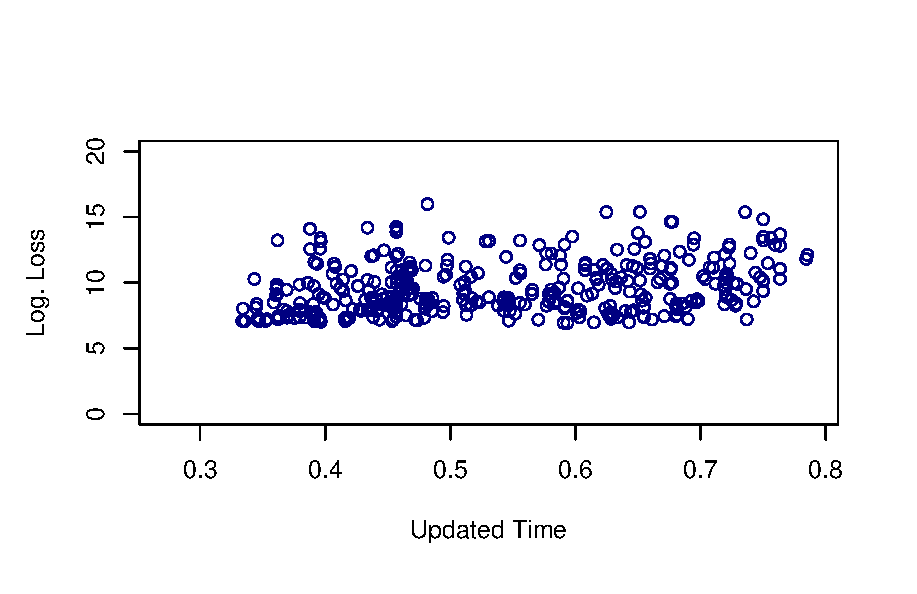
\includegraphics[width=7.5cm]{IntraDayUpdatedTime.eps}
         &
         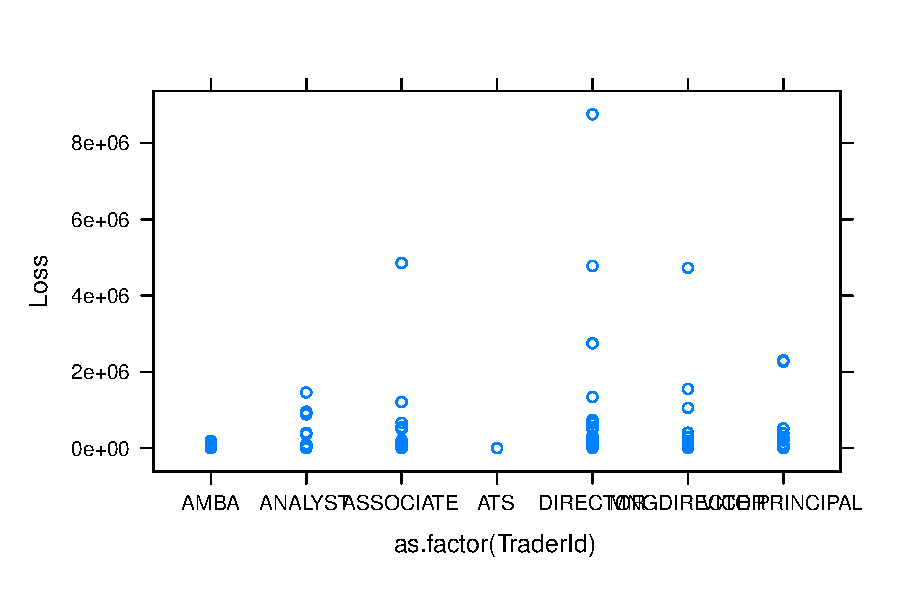
\includegraphics[width=7cm]{TrendTraderId.eps}
         \end{tabular}
    \end{frame}
\subcaption{Scatterplots}
   \label{Intra_Day_Trends} 
\end{subfigure}

\begin{subfigure}[b]{0.55\textwidth}
   \begin{frame}
      \centering
       \begin{tabular}{cc}
        \textbf{Loss per month} & \textbf{Trading frequency} \\
        \includegraphics[width=7.5cm]{UpdatedDayFreq.eps}
         &
         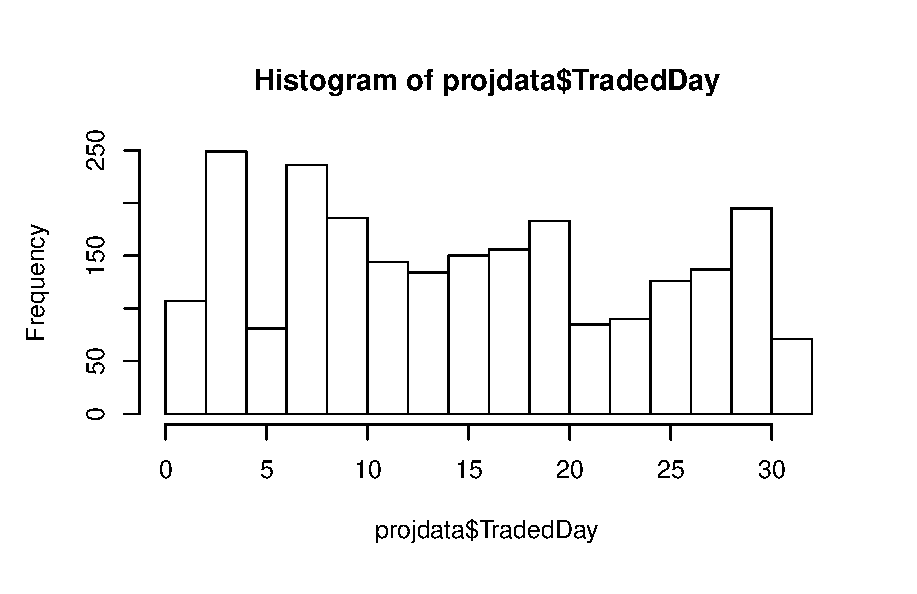
\includegraphics[width=7cm]{TradedDayFreq.eps}
         \end{tabular}
    \end{frame}
\subcaption{Histograms}
   \label{Hist_Loss_Freq}
\end{subfigure}
\caption[Numerical grid display]{(a) Scatterplots of intra-day trend analysis for logs of severities of operational events and trends incident activity for identifying the role of the trader originating the incidents. (b) As for (a) but in the form of histograms showing the frequency distrbution of the number daily operational indicents and the number of trades over a monthly period.} 
\end{figure}

\subsection{Characteristics of exposure}

The exposure of risk of type \(i\), \(d_i\) shows the daily duration,
from when the trade was booked to the moment the operational risk event
was observed and ended. This measure is defined this way when
specifically applied to projecting the number of loss events
(frequencies) and can be plotted as follows depicted in graphs depicted
in Figure \ref{Exploration_analysis_exposure}.\medskip

\begin{figure}
\begin{frame}
      \centering
       \begin{tabular}{ccc}
        \textbf{Distribution} & \textbf{Density} & \textbf{Digital Analysis} \\
        \includegraphics[width=5cm]{Exposure_cdf.eps}
         &
         \includegraphics[width=5cm]{Dist_exposure.eps}
         &
         \includegraphics[width=5cm]{Benford.eps}
         \end{tabular}
    \end{frame}
        \captionof{figure}{A simple comparison of the Sigmoidal like features of the fat-tailed, right skewed distribution for exposure, and first-digit frequency distribution from the exposure data with the expected distribution according to Benford's Law}
    \label{Exploration_analysis_exposure}
\end{figure}

The variable follows a logistic trend on \([0,1]\), implying an FIs
operational risk portfolio rises like a sigmoid function throughout the
period of observation, typically starting from \(0\), which then
observes a plateau in growth. The average exposure is 389.99 or about 1
year.\medskip

Grid plots \ref{Exploration_analysis_exposure} portray the logistic
function, together with a simple comparison of first-digit frequency
distribution analysis, according to Benford's Law, with exposure data
distribution. The close fitting nature implies the data are uniformly
distributed across several orders of magnitude, especially within the 1
year period.\medskip

\subsection{Characteristics of the covariates}

The characteristics of the operational risk portfolio are given by the
following covariates: \emph{UpdatedDay}, \emph{UpdatedTime} - the day of
the month and time of day the OpRisk incident occurs respectively;
\emph{TradedDay}, \emph{TradedTime} - the day in the month and time of
day the deal was originated respectively; The \emph{LossIndicator} as
indicated before is a binary variable consisting of two values: A \(0\),
which indicates pending or near misses, and \(1\), if the incident
results in a realised loss, meaning that there is significant p\&L
impact due to the OpRisk incident.\medskip

the \emph{Desk} is the location in the portfolio tree the incident
originated, it is a factor variable conisting of 10 categories;
\emph{CapturedBy}, the designated analyst who actions the incident, a
factor variable consisting of 5 categories; \emph{TraderId}, the trader
who originates the deal, a factor variable with 7 categories;
\emph{TradeStatus}, the live status of the deal, a factor variable with
4 categories; \emph{Instrument}, the type of deal, a factor variable
with 23 categories; \emph{Reason}, a description of the cause of the
OpRisk incident, a factor variable with 19 levels;
\emph{EventTypeCategoryLevel}, 7 OpRisk event types as per Risk (2001),
a factor variable with 5 categories; \emph{BusinessLineLevel}, 8 OpRisk
business lines as per Risk (2001), a factor variable with 8
categories.\medskip

\singlespacing

\doublespacing

The continuous numerical variable \emph{Loss}, shows the financial
impact (severity) of the OpRisk incident in Rands. For the most part
(i.e.~96.1\% of the time) OpRisk incidents result in pending losses
and/or near misses, most realised losses (2.3\%) lie within the
{[}\textbf{R$200,00$}, \textbf{R$300,000$}{]} range. In the current
portfolio there are also five p\&L impacts higher than
\textbf{R$2.5$ million}.\medskip

\subsection{Characteristics of daily operational activity}

The distribution of daily losses and/or pending/near misses by
operational activities are represented in
\ref{Exploratory_Time_Day_Frequency3plot}. Figure
\ref{Exploratory_UpdateTime_Frequency3plot} shows that most operational
events occur in times leading up to midday (i.e.~10:50AM to 11:50AM),
the observed median is 11:39AM, and of these potential loss events, most
realised losses occur closest to mid-day. The frequencies of the loss
incidents in the analysed portfolio sharply decreases during the
following period, i.e.~from 12:10PM to 13:10PM, during which the least
realised losses occur.\medskip

Figure \ref{Exploratory_UpdateDay_Frequency3plot} shows that operational
activity increases in intensity in the days leading up to the middle of
the month, i.e.~\(10^{th}\) - \(15^{th}\); the observed mean is
\(14.49\) days, and of these potential loss events, realised losses
especially impact on the portfolio during these days.

\singlespacing

\doublespacing

\begin{figure}
\centering
\begin{subfigure}[b]{0.55\textwidth}
   \includegraphics[width=1.5\linewidth]{Exploratory_UpdateTime_Frequency3plot.eps}
   \subcaption{Frequency distributions of operational incidents by the time in the day}
   \label{Exploratory_UpdateTime_Frequency3plot} 
\end{subfigure}

\begin{subfigure}[b]{0.55\textwidth}
   \includegraphics[width=1.5\linewidth]{Exploratory_UpdateDay_Frequency3plot.eps}
   \subcaption{Frequency distributions of operational incidents by the day in the month}
   \label{Exploratory_UpdateDay_Frequency3plot}
\end{subfigure}

\caption[Two numerical solutions: Histograms showing the distribution of UpdatedTime \& UpdatedDay by LossIndicator.]{The frequency distributions of All the losses, the realised losses, and pending/near misses of operational incidents by the day in the month when the indidents' occurred}
\label{Exploratory_Time_Day_Frequency3plot}
\end{figure}

Similarly, the influence of trading desk's on the frequency of
operational events can be analysed on the basis of the portfolio's
bidimensional distribution by variables \emph{Desk} and
\emph{LossIndicator}, which shows the proportions realised losses vs
pending and/or near misses for each particular desk. The bidimensional
distribution of \emph{Desk} and \emph{LossIndicator} is presented in a
contingency table, Table \ref{tab_Desk_Prop}, in which it's considered
useful to calculate proportions for each desk category.

\begin{figure}
\centering
\includegraphics[width=15cm,height=5cm]{Density_UpdateDay_TradedDay.eps}
\caption[Density plots showing a comparison of realised vs pending losses and/near misses over a month for the day in the month the OpRisk incident was updated to the day in the month trades were traded/booked]{Density plots showing a comparison of realised vs pending losses and/near misses over a month for the day in the month the OpRisk incident was updated to the day in the month trades were traded/booked}
\label{Desk_Proportions}
\end{figure}

\singlespacing

\doublespacing

\begin{table}[ht]
\centering
\caption{Occurence of realised losses: proportions on desk categories}
\begin{tabular}{lccr}
\toprule
  & \multicolumn{3}{c}{No. of transactions} \\
Desk   & no Loss   & Loss & Total\\ 
\midrule
  Africa            &  49 & 10 &  59 \\
  Bonds/Repos       & 113 & 31 & 144 \\
  Commodities       & 282 & 45 & 327 \\
  Derivatives       & 205 & 24 & 229 \\
  Equity            & 269 & 66 & 335 \\
  Management/Other  &  41 &  2 &  43 \\
  Money Market      & 169 & 52 & 221 \\
  Prime Services    & 220 & 62 & 282 \\
  Rates             & 336 & 53 & 389 \\
  Structured Notes  & 275 & 26 & 301 \\
 \bottomrule
\end{tabular}\label{tab_Desk_Prop}
\end{table}

Thus, as illustratred in figure \ref{Desk_Proportions}, from 23,5\%; the
highest proportion of realised losses per desk is the Money Market (MM)
desk, the figures are decreasing, followed by Prime Services (22\%);
Bonds/Repos (21,5\%); Equity (19,7\%); Africa (16,9\%); Commodities
(13,8\%); Rates (13,6\%); Derivatives (10,5\%); Structured Notes (SND)
(8.6\%), to the least proportion in the Management/Other, a category
where only 4,7\% of operations activities were realised as losses.

\singlespacing

\doublespacing

\begin{figure}
\centering
\includegraphics[width=15cm,height=5cm]{Exploratory_Desk_Proportions.eps}
\caption[Desk category by realised losses]{Histograms showing the proportions of realised losses vs all losses including pending and/or near misses by desk category}
\label{Desk_Proportions}
\end{figure}

This behaviour can be extended beyond the trading desk, as represented
in Figure \ref{Mosaic_Instr_Trd_Tec}, a mosaic plot grid presenting the
structure of the OpRisk portfolio by Instrument, TraderId, CapturedBy
\footnote{i.e. the type of financial instrument, the trader who originated the incident on the deal, and the role of the technical support personnel who is involved in the query resolution.}
and the operational losses.

\singlespacing

\doublespacing

\begin{figure}
\begin{frame}
      \centering
       \begin{tabular}{cc}
        \textbf{Type of instrument traded} & \textbf{Role identification} \\
        \includegraphics[width=7.5cm,height=15cm]{Single_Instr.eps}
         &
         \includegraphics[width=7.5cm,height=15cm]{Stacked_TrId_TechSup.eps}
         \end{tabular}
    \end{frame}
    \caption{Mosaic grid plots for the bidimensional distribution by traded instrument, the trader originating the operational event, and by the technical support personnel involved in query resolution, against the dummy variable showing if a realised loss was reported.}
    \label{Mosaic_Instr_Trd_Tec}
\end{figure}

One can notice that the width of the bars corresponding to the different
categories, i.e.~Instrument, TraderId, CapturedBy, is given by their
proportion in the sample. In particular, for the category `at least one
realised loss', in the top right mosaic of Figure
\ref{Mosaic_Instr_Trd_Tec} portrays a increase in ``riskiness'' trending
up from Associate to AMBA, Analyst, Vice Principal, Managing Director,
Director, up to the risky ATS category, which are automated trading
system generated trades.\medskip

Figure \ref{Mosaic_Instr_Trd_Tec} bottom right mosaic plot for technical
support personnel for the category `at least one realised loss',
portrays a downward trend, slowing in riskiness from Unauthorised User
downward to Tech Support, Mid Office, Prod Controller down to the least
risky Prod Accountant. This intepretation makes sense given unauthorised
users are more likely to make impactful operational errors, technical
support personnel would also be accountable for large impacts albiet for
contrasting reasons, they are mandated to perform these deal adjustments
which have unavoidable impacts associated with them, whereas the former
group are unauthorised to perform adjustments therefore may lack the
skill, or be criminally minded insiders acting on their own or in unison
to enable their underhanded practices and intentions without raising any
suspicion.\medskip   

\begin{table}[!htbp] \centering 
  \caption{Summary statistics for all losses as per Instrument type} 
  \label{Stargazer} 
\begin{tabular}{@{\extracolsep{5pt}}lccccccc} 
\\[-1.8ex]\hline 
\hline \\[-1.8ex] 
Statistic & \multicolumn{1}{c}{N} & \multicolumn{1}{c}{Mean} & \multicolumn{1}{c}{St. Dev.} & \multicolumn{1}{c}{Min} & \multicolumn{1}{c}{Pctl(25)} & \multicolumn{1}{c}{Pctl(75)} & \multicolumn{1}{c}{Max} \\ 
\hline \\[-1.8ex] 
Mean & 23 & 34,603 & 46,007 & 306 & 7,697 & 44,157 & 192,513 \\ 
\hline \\[-1.8ex] 
\end{tabular} 
\end{table}

In another mosaic plot, Figure \ref{Mosaic_Contingency}, the
bidimensional distribution of transactions by trader and realised vs
pending losses, conditional on the trade status is presented and
analysed. Here, and in the contingency table, Table
\ref{tab:Mosaic_Contingency}, we can clearly see the following trends:
In BO-BO confirmed status - an increase in realised losses from the
leftmost TraderID (i.e.~AMBA) to right, and the opposite for
transactions performed in BO Confirmed status (both with two
exceptions). In particular, the biggest number of realised losses in
both BO and BO-BO Confirmed statuses occur due to automated trading
systems (ATS) who also give rise to the exceptions mentioned.\medskip

Table \ref{tab:Mosaic_Contingency} and Figure \ref{Mosaic_Contingency}
are obtained with the following commands:

\singlespacing

\singlespacing
\begin{figure}
\centering
\textbf{Mosasic plot for trader identification and loss indicator, by trade status}
\includegraphics[width=\linewidth,height=0.75\linewidth]{Mosaic_Contingency.eps}
\caption[Portfolio structure by trader, trade status and number of realised losses]{A mosaic plot representing the structure of the operational risk portfolio by trader identification (TraderId), the status ofthe trade (TradeStatus) and the number of realised losses vs pending or near misses}
\label{Mosaic_Contingency}
\end{figure}
\doublespacing

Table \ref{tab:Crosstab_covariate} presents the most frequent category
in the operational risk dataset for each possible covariate.

\begin{table}[htbp]
        \centering
        \textbf{Crosstab of trader identification and loss indicator, by trade status}
\singlespacing        
        \small
        \setlength\tabcolsep{2pt}
            \begin{tabular}{|p{2cm}|p{2cm}|l|l|l|l|l|l|p{2cm}|p{2cm}|} \hline
            & & \multicolumn{7}{|c|}{Trader Identification} \\ \hline
            TradeStatus & Loss Indicator & Amba & Analyst & Associate & ATS & Director & Mng Director & Vice Principal \\\hline
            \multirow{2}{*}{BO-BO Confirmed} & 0 & 24 & 136 & 320 & 0 & 282 & 52 & 49 \\ \cline{2-9}
                                   & 1 & 2  &  15 & 43 & 0 & 50 & 18 & 16 \\\cline{2-9}
            \multirow{2}{*}{BO Confirmed} & 0 & 17  & 299 & 153 & 13 & 257 & 102 & 153 \\ \cline{2-9}
                                   & 1 &  3 &  71 & 12 & 8 &  62 & 23 & 30 \\ \cline{2-9}
            \multirow{2}{*}{Terminated}       & 0 & 83 & 9 & 1 & 0 & 0 & 2 & 1 \\ \cline{2-9}
                                  & 1 & 17 & 1 & 0 & 0 & 0 & 0 & 0 \\ \cline{2-9}
            \multirow{2}{*}{Terminated/Void}  & 0 & 2 & 0 & 0 & 0 & 2 & 1 & 1 \\ \cline{2-9}
                                   & 1 & 0 & 0 & 0 & 0 & 0 & 0 & 0 \\ \hline
            \end{tabular}
            \caption{A contingency table showing the bidimensional distribution of transactions by trader identification vs realised and/or pending losses, conditional on the trade status}
            \label{tab:Crosstab_covariate}
\end{table}
\doublespacing

\begin{table}[htbp]
        \centering
        \textbf{Modal classes for the categorical variables} 
\singlespacing        
        \small
        \setlength\tabcolsep{2pt}
            \begin{tabular}{|l|l|p{4cm}|} \hline
            Variable & Modal class or category & Name of modal class \\\hline
            Desk & Rates & DeskRates \\ \cline{1-3}
            CapturedBy & TECHSUPPORT & CapturedBy\_TECHSUPPORT \\ \cline{1-3}
            TradeStatus & BO confirmed & TradeStatus\_BO confirmed \\ \cline{1-3}
            TraderId & DIRECTOR & TraderId\_DIRECTOR \\ \cline{1-3}
            Instrument & Swap & Instrument\_Swap \\ \cline{1-3}
            Reason & Trade enrichment for system flow  & Reason\_Trade enrichment for system flow \\ \cline{1-3}
            EventTypeCategoryLevel & EL7 & EventTypeCategoryLevel\_EL7 \\ \cline{1-3}
            BusinessLineLevel & BL2 & BusinessLineLevel\_BL2 \\ \cline{1-3} 
            \end{tabular}
            \caption{A contingency table showing the bidimensional distribution of transactions by trader identification vs realised and/or pending losses, conditional on the trade status}
            \label{tab:Mosaic_Contingency}
\end{table}
\doublespacing

\section{The estimation of some poisson regression generalised linear models (GLM's)}
\label{sec:The estimation of some poisson regression generalised linear models (GLM's)}

\singlespacing

\FloatBarrier
\newpage
\fancyhead[L]{Chapter 4's Title}
\fancyhead[R]{\thepage}
\fancyfoot[C]{}

\chapter{Chapter 4's Title}

\FloatBarrier
\newpage
\fancyhead[L]{Chapter 5's Title}
\fancyhead[R]{\thepage}
\fancyfoot[C]{}

\chapter{Chapter 5's Title}

\FloatBarrier
\newpage
\fancyhead[L]{References}
\fancyhead[R]{\thepage}
\fancyfoot[C]{}

\chapter*{REFERENCES}

\setlength{\parindent}{-0.5in}
\setlength{\leftskip}{0.4in}
\setlength{\parskip}{6pt}

\noindent

\hypertarget{refs}{}
\leavevmode\hypertarget{ref-acharyya2012current}{}%
Acharyya, M. (2012). Why the current practice of operational risk
management in insurance is fundamentally flawed: Evidence from the
field. \emph{ERM symposium, april}, 18--20.

\leavevmode\hypertarget{ref-agostini2010combining}{}%
Agostini, A., Talamo, P., \& Vecchione, V. (2010). Combining operational
loss data with expert opinions through advanced credibility theory.
\emph{The Journal of Operational Risk}, \emph{5}(1), 3.

\leavevmode\hypertarget{ref-altman2008behavioral}{}%
Altman, M. (2008). \emph{Behavioral economics, economic theory and
public policy}.

\leavevmode\hypertarget{ref-aue2006lda}{}%
Aue, F., \& Kalkbrener, M. (2006). LDA at work: Deutsche bank's approach
to quantifying operational risk. \emph{Journal of Operational Risk},
\emph{1}(4), 49--93.

\leavevmode\hypertarget{ref-badescu2015modeling}{}%
Badescu, A. L., Lan, G., Lin, X. S., \& Tang, D. (2015). \emph{Modeling
correlated frequencies with application in operational risk management}.

\leavevmode\hypertarget{ref-barberis2003survey}{}%
Barberis, N., \& Thaler, R. (2003). A survey of behavioral finance.
\emph{Handbook of the Economics of Finance}, \emph{1}, 1053--1128.

\leavevmode\hypertarget{ref-cameron2013regression}{}%
Cameron, A. C., \& Trivedi, P. K. (2013). \emph{Regression analysis of
count data} (Vol. 53). Cambridge university press.

\leavevmode\hypertarget{ref-chau2014robust}{}%
Chau, V. (2014). \emph{Robust estimation in operational risk modeling}
(Master's thesis).

\leavevmode\hypertarget{ref-chavez2016extreme}{}%
Chavez-Demoulin, V., Embrechts, P., \& Hofert, M. (2016). An extreme
value approach for modeling operational risk losses depending on
covariates. \emph{Journal of Risk and Insurance}, \emph{83}(3),
735--776.

\leavevmode\hypertarget{ref-chavez2006quantitative}{}%
Chavez-Demoulin, V., Embrechts, P., \& Nešlehová, J. (2006).
Quantitative models for operational risk: Extremes, dependence and
aggregation. \emph{Journal of Banking \& Finance}, \emph{30}(10),
2635--2658.

\leavevmode\hypertarget{ref-basel2010basel}{}%
Committee, B., \& others. (2010). Basel iii: A global regulatory
framework for more resilient banks and banking systems. \emph{Basel
Committee on Banking Supervision, Basel}.

\leavevmode\hypertarget{ref-basel2011operational}{}%
Committee, B., \& others. (2011). Operational risk--supervisory
guidelines for the advanced measurement approaches. \emph{Basel: Bank
for International Settlements}.

\leavevmode\hypertarget{ref-covrig2015using}{}%
Covrig, M., Mircea, I., Zbaganu, G., Coser, A., Tindeche, A., \& others.
(2015). Using r in generalized linear models. \emph{Romanian Statistical
Review}, \emph{63}(3), 33--45.

\leavevmode\hypertarget{ref-cruz2002modeling}{}%
Cruz, M. G. (2002). \emph{Modeling, measuring and hedging operational
risk}. John Wiley \& Sons New York,

\leavevmode\hypertarget{ref-de2008generalized}{}%
De Jong, P., \& Heller, G. Z. (2008). \emph{Generalized linear models
for insurance data}. Cambridge University Press.

\leavevmode\hypertarget{ref-denuit2007actuarial}{}%
Denuit, M., Maréchal, X., Pitrebois, S., \& Walhin, J.-F. (2007).
\emph{Actuarial modelling of claim counts: Risk classification,
credibility and bonus-malus systems}. John Wiley \& Sons.

\leavevmode\hypertarget{ref-dobson2008introduction}{}%
Dobson, A. J., \& Barnett, A. (2008). \emph{An introduction to
generalized linear models}. Chapman; Hall/CRC.

\leavevmode\hypertarget{ref-mysis2013}{}%
Dorval, M. (2013). \emph{Achieving Basel III compliance: how to tackle
it and business issues} (pp. 1--12). Retrieved from
\url{http://www.risktech-forum.com/research/achieving-basel-iii-compliance-how-to-tackle-it-and-business-issues}

\leavevmode\hypertarget{ref-einemann2018operational}{}%
Einemann, M., Fritscher, J., \& Kalkbrener, M. (2018). \emph{Operational
risk measurement beyond the loss distribution approach: An
exposure-based methodology}.

\leavevmode\hypertarget{ref-embrechts2002correlation}{}%
Embrechts, P., McNeil, A., \& Straumann, D. (2002). Correlation and
dependence in risk management: Properties and pitfalls. \emph{Risk
Management: Value at Risk and Beyond}, \emph{1}, 176--223.

\leavevmode\hypertarget{ref-embrechts2018modeling}{}%
Embrechts, P., Mizgier, K. J., \& Chen, X. (2018). \emph{Modeling
operational risk depending on covariates. An empirical investigation.}

\leavevmode\hypertarget{ref-frachot2001loss}{}%
Frachot, A., Georges, P., \& Roncalli, T. (2001). \emph{Loss
distribution approach for operational risk}.

\leavevmode\hypertarget{ref-frees2010household}{}%
Frees, E. W., \& Sun, Y. (2010). Household life insurance demand: A
multivariate two-part model. \emph{North American Actuarial Journal},
\emph{14}(3), 338--354.

\leavevmode\hypertarget{ref-friedman1948utility}{}%
Friedman, M., \& Savage, L. J. (1948). The utility analysis of choices
involving risk. \emph{Journal of Political Economy}, \emph{56}(4),
279--304.

\leavevmode\hypertarget{ref-galloppo2014review}{}%
Galloppo, G., \& Previati, D. (2014). \emph{A review of methods for
combining internal and external data}.

\leavevmode\hypertarget{ref-gigerenzer2009homo}{}%
Gigerenzer, G., \& Brighton, H. (2009). Homo heuristicus: Why biased
minds make better inferences. \emph{Topics in Cognitive Science},
\emph{1}(1), 107--143.

\leavevmode\hypertarget{ref-hemrit2012major}{}%
Hemrit, W., \& Arab, M. B. (2012). The major sources of operational risk
and the potential benefits of its management. \emph{The Journal of
Operational Risk}, \emph{7}(3), 71--92.

\leavevmode\hypertarget{ref-hoohlo2015new}{}%
Hoohlo, M. (2015). \emph{A new internal data measure for operational
risk: A case study of a south african bank} (PhD thesis).

\leavevmode\hypertarget{ref-de2015combining}{}%
Jongh, R. de, De Wet, T., Raubenheimer, H., \& Venter, J. H. (2015).
\emph{Combining scenario and historical data in the loss distribution
approach: A new procedure that incorporates measures of agreement
between scenarios and historical data}.

\leavevmode\hypertarget{ref-kahneman2003perspective}{}%
Kahneman, D. (2003). A perspective on judgment and choice: Mapping
bounded rationality. \emph{American Psychologist}, \emph{58}(9), 697.

\leavevmode\hypertarget{ref-kahneman2013prospect}{}%
Kahneman, D., \& Tversky, A. (2013). Prospect theory: An analysis of
decision under risk. In \emph{Handbook of the fundamentals of financial
decision making: Part i} (pp. 99--127). World Scientific.

\leavevmode\hypertarget{ref-king2001operational}{}%
King, J. L. (2001). \emph{Operational risk: Measurement and modelling
(the wiley finance series)}.

\leavevmode\hypertarget{ref-kuhnen2005neural}{}%
Kuhnen, C. M., \& Knutson, B. (2005). The neural basis of financial risk
taking. \emph{Neuron}, \emph{47}(5), 763--770.

\leavevmode\hypertarget{ref-list2004neoclassical}{}%
List, J. A. (2004). Neoclassical theory versus prospect theory: Evidence
from the marketplace. \emph{Econometrica}, \emph{72}(2), 615--625.

\leavevmode\hypertarget{ref-mignola2016comments}{}%
Mignola, G., Ugoccioni, R., \& Cope, E. (2016). \emph{Comments on the
basel committee on banking supervision proposal for a new standardized
approach for operational risk}.

\leavevmode\hypertarget{ref-morgenstern1953theory}{}%
Morgenstern, O., \& Von Neumann, J. (1953). \emph{Theory of games and
economic behavior}. Princeton university press.

\leavevmode\hypertarget{ref-nelder1972generalized}{}%
Nelder, J. A., \& Wedderburn, R. W. (1972). Generalized linear models.
\emph{Journal of the Royal Statistical Society: Series A (General)},
\emph{135}(3), 370--384.

\leavevmode\hypertarget{ref-opdyke2014estimating}{}%
Opdyke, J. D. (2014). Estimating operational risk capital with greater
accuracy, precision, and robustness. \emph{arXiv Preprint
arXiv:1406.0389}.

\leavevmode\hypertarget{ref-panjer2006operational}{}%
Panjer, H. H. (2006). \emph{Operational risk: Modeling analytics} (Vol.
620). John Wiley \& Sons.

\leavevmode\hypertarget{ref-parodi2014pricing}{}%
Parodi, P. (2014). \emph{Pricing in general insurance}. CRC Press.

\leavevmode\hypertarget{ref-peters2016should}{}%
Peters, G., Shevchenko, P. V., Hassani, B., \& Chapelle, A. (2016).
\emph{Should the advanced measurement approach be replaced with the
standardized measurement approach for operational risk?}

\leavevmode\hypertarget{ref-risk2001supporting}{}%
Risk, B. O. (2001). Supporting document to the new basel capital accord.
\emph{Consultative Document, January}, \emph{200}.

\leavevmode\hypertarget{ref-risk2016supporting}{}%
Risk, B. O. (2016). Standardised measurement approach for operational
risk. \emph{Consultative Document, June}.

\leavevmode\hypertarget{ref-shefrin2016behavioral}{}%
Shefrin, H. (2016). \emph{Behavioral risk management: Managing the
psychology that drives decisions and influences operational risk}.
Springer.

\leavevmode\hypertarget{ref-tom2007neural}{}%
Tom, S. M., Fox, C. R., Trepel, C., \& Poldrack, R. A. (2007). The
neural basis of loss aversion in decision-making under risk.
\emph{Science}, \emph{315}(5811), 515--518.

\leavevmode\hypertarget{ref-urbina2014application}{}%
Urbina, J., \& Guillén, M. (2014). An application of capital allocation
principles to operational risk and the cost of fraud. \emph{Expert
Systems with Applications}, \emph{41}(16), 7023--7031.

\leavevmode\hypertarget{ref-wiseman1997longitudinal}{}%
Wiseman, R. M., \& Catanach Jr, C. (1997). A longitudinal disaggregation
of operational risk under changing regulations: Evidence from the
savings and loan industry. \emph{Academy of Management Journal},
\emph{40}(4), 799--830.

\leavevmode\hypertarget{ref-wood2017generalized}{}%
Wood, S. N. (2017). \emph{Generalized additive models: An introduction
with r}. Chapman; Hall/CRC.

\bibliography{Thesis.bib}


\end{document}
